 \documentclass[structabstract]{aa}

\usepackage{natbib}
\usepackage{graphicx}
\usepackage{epstopdf}
\usepackage{color}
\usepackage{hyperref}
\hypersetup{colorlinks, citecolor=blue, filecolor=black, linkcolor=black, urlcolor=black}


\newcommand{\vdag}{(v)^\dagger}
\newcommand{\myemail}{jbyrne@ifa.hawaii.edu}

%%I'm adding these -JPB
%\newcommand{\solphys}{{\it Solar Physics}}
%\newcommand{\aap}{    {\it Astronomy \& Astrophysics}}
%\newcommand{\aaps}{   {\it Astronomy \& Astrophysics Supplemental}}
%\newcommand{\apj}{    {\it Astrophysical Journal}}
%\newcommand{\apjl}{    {\it Astrophysical Journal Letters}}
%\newcommand{\jgr}{    {\it Journal of Geophysical Research}}
%\newcommand{\aapr}{    {\it Astronomy \& Astrophysics Review}}
%\newcommand{\grl}{    {\it Geophysical Research Letters}}
\newcommand{\lrsp}{    {\it Living Rev. Solar Phys.}}
\newcommand{\stat}{Ann. Stat.}

\newcommand{\RNum}[1]{\uppercase\expandafter{\romannumeral #1\relax}}

\usepackage{subfigure}

%\makeatletter
%\newcommand*{\rom}[1]{\expandafter\@slowromancap\romannumeral #1@}
%\makeatother


\begin{document}

\title{Improved methods for determining the kinematics of coronal mass ejections and coronal waves.}

\titlerunning{Improved methods for determining the kinematics of CMEs and coronal waves.}
\authorrunning{Byrne et al.}

\author{J.\,P.\,Byrne\inst{1}
	\and D.\,M.\,Long\inst{2}
	\and P.\,T.\,Gallagher\inst{3}
	\and D.\,S.\,Bloomfield\inst{3}
	\and S.\,A.\,Maloney\inst{4}
	\and R.\,T.\,J.\,McAteer\inst{5}
	\and H.\,Morgan\inst{6,1,7}
	\and S.\,R.\,Habbal\inst{1}
	}
\institute{Institute for Astronomy, University of Hawai'i, 2680 Woodlawn Drive, Honolulu, HI 96822, USA.\\
		\email{jbyrne@ifa.hawaii.edu}
		\and
		UCL--Mullard Space  Science Laboratory, Holmbury St. Mary, Dorking, Surrey, RH5 6NT, UK.
		\and 
		School of Physics, Trinity College Dublin, College Green, Dublin 2, Ireland.
		\and
		Skytek, 51/52 Fitzwilliam Square West, Dublin 2, Ireland
		\and
		Department of Astronomy, New Mexico State University, Las Cruces, NM 88003-8001, USA.
		\and
		Sefydliad Mathemateg a Ffiseg, Prifysgol Aberystwyth, Ceredigion, Cymru, SY23 3BZ.
		\and
		Coleg Cymraeg Cenedlaethol, Y Llwyfan, Ffordd y Coleg, Caerfyrddin, Cymru, SA31 3EQ.
		}

\date{Received ?; accepted ?}
%%Abstract
\abstract
% Context (optional)
{The study of solar eruptive events and associated phenomena is of great importance in the context of solar and heliophysics. Coronal mass ejections (CMEs) and coronal waves are energetic manifestations of the restructuring of the solar magnetic field and mass motion of the plasma. Characterising this motion is vital for deriving the dynamics of these events and thus understanding the physics driving their initiation and propagation. The development and use of appropriate methods for measuring event kinematics is therefore imperative.} 
% Aims (mandatory)
{Traditional approaches to the study of CME and coronal wave kinematics do not return wholly accurate nor robust estimates of the true event kinematics and associated uncertainties. We highlight the drawbacks of these approaches, and demonstrate improved methods for accurate and reliable determination of the kinematics.}
% Methods (mandatory)
{We discuss the limitations of traditional numerical differentiation techniques when applied to small data-sets. The Savitzky-Golay filter is demonstrated as a more appropriate fitting technique for CME and coronal wave studies, and a residual resampling bootstrap technique is demonstrated as a statistically rigorous method for the determination of kinematic error estimates and goodness-of-fit tests.}
% Results (mandatory)
{It is shown that the scatter on distance-time measurements of small sample size can significantly limit the ability to derive accurate and reliable kinematics. This may be overcome by (\emph{i}) increasing measurement precision and sampling cadence, and (\emph{ii}) by applying robust methods for deriving the kinematics and reliably determining their associated uncertainties. If a priori knowledge exists, as it does in this case, and a pre-determined model form for the kinematics (or indeed any justified fitting-form to be tested against the data) is available, then its accuracy can be examined using a bootstrapping technique to determine the confidence interval associated with the model/fitting parameters.}
% Conclusions (optional)
{Improved methods for determining the kinematics of CMEs and coronal waves are demonstrated to great effect, overcoming many issues highlighted in traditional numerical differencing and error propagation techniques.}

%% Keywords 

\keywords{Sun: activity -- Sun: corona -- Sun: coronal mass ejections (CMEs) -- Methods: data analysis -- Methods: numerical -- Methods: statistical}

\maketitle

%
%________________________________________________________________

\section{Introduction}
\label{sect_intro}

% Set the scene
Coronal mass ejections (CMEs) and coronal waves (commonly known as ``EIT waves") are large-scale manifestations of solar activity that indicate a restructuring of the global solar magnetic field. These phenomena involve the mass motion of plasma through the solar corona, with energies on the order of $10^{25}\,J$ for CMEs \citep{2004JGRA..10910104E}, and upwards of $10^{18}\,J$ for coronal waves \citep{2005ApJ...633L.145B}. CME speeds range from about 20 to $>$$2500\,km\,s^{-1}$ \citep{2004JGRA..10907105Y}, most typically moving at speeds akin to those of coronal waves, which range from 50 to $>$$700\,km\,s^{-1}$ \citep{2009ApJS..183..225T}. Observational catalogues of these events have been compiled from over $\sim$20\,years of observations, with the aim of characterizing their physical properties in order to better understand the dynamics of their initiation and propagation \citep[see some recent reviews by][]{2011SSRv..158..365G,2012SoPh..tmp...93P,2011ASSL..376.....H,2012LRSP....9....3W}. CME dynamics, in particular, are of great interest in a space weather context \citep[e.g.,][]{SWE:SWE493, 2010heliophysics, 2005A&A...440..373H}. Therefore methods for determining their kinematics with improved accuracy are extremely important if scientists are to become skilled at predicting their behavior and arrival times \citep[see, for example, efforts by][]{2010NatCo...1E..74B, 2005AnGeo..23.1033S, 2004Natur.432...78P}. \citet{2012ApJ...749...57T} also highlight the importance of characterizing kinematics of events as accurately as possible, in order to understand the effects of drag and CME-CME interactions, and the subsequent implications for the underlying magnetic field structures involved.

In order to observe and characterize the motion of the bulk plasma of these events, a method of image-differencing is traditionally used, whereby a preceding image is subtracted from a leading image in order to highlight moving features. However, this approach enhances relative rather than actual motion, and is prone to spatiotemporal crosstalk and user-dependent bias. More recent work has used single-image processing techniques such as multiscale filters \citep{2011AdSpR..47.2118G, 2009A&A...495..325B, 2008SoPh..248..457Y} and robust automated approaches \citep[e.g.,][]{2012ApJ...752..145B, 2012SoPh..276..479P, 2011A&A...531A..42L} to overcome these issues and reveal the true physical characteristics of the events. Thus by accurately tracking the position of a feature over time, it is possible to determine the kinematics of the event. 

The true physical nature of coronal waves is not fully understood, with two main competing theories: that they are indeed waves \citep[e.g.,][]{2012ApJ...754....7S,2010ApJ...716L..57V}, or that they are signatures of magnetic field restructuring during a CME eruption \citep[e.g.,][]{2011ApJ...738..167S,2011ApJ...732L..20C}. Their kinematic behavior has been proposed as one of the main discriminators between these competing theories, with the relatively high velocities measured thus far suggesting a wave interpretation to be appropriate \citep{2012ApJ...753..112Z, 2011A&A...532A.151W}. Similarly, the low-coronal kinematics of CMEs may be used to discriminate between eruption mechanisms \citep[see, for example,][and the CME models discussed therein]{2010A&A...516A..44L}. However \citet{2007ApJ...657.1117W} demonstrate that the errors in CME acceleration values can be of the same order as the accelerations typically measured, making this task difficult. This has led to many statistical studies employing large numbers of events to try and glean a general form for typical CME motion \citep[e.g.,][]{2006ApJ...649.1100Z, 2003AdSpR..32.2637D, 2000GeoRL..27..145G}. However, individual events need to be studied with rigor in order to satisfactorily derive the kinematics, and gain insight to the physics at play.

A variety of different mathematical techniques exist for deriving the kinematics of transient features, most being based upon some form of numerical differentiation of the distance-time measurements, and/or the fitting of a pre-assumed model function. While such techniques may appear mathematically sound, some of them are not necessarily applicable to the derivation of kinematics for these specific events, and can produce spurious results. \citet{2010ApJ...712.1410T} demonstrated the applicability of an inversion technique (developed by \citealt{2005SoPh..227..299K}) to overcome some of these issues. They highlight its effectiveness at reducing the errors on three CME/flare studies, compared to a standard spline-fit approach, and so the technique shows promise if it can be applied robustly across many various events. Here, we further explore improved methods for overcoming the issues outlined above, to robustly determine the kinematics of CMEs and coronal waves with improved accuracy and reliability.

A review of standard numerical methods and error propagation are presented in Section~\ref{sect:num_diff_errors}. Simulations of the drawbacks of a standard numerical derivative are presented in Section~\ref{sect:simul1}. In Section~\ref{sect:bootstrapping} we outline a more appropriate method for inspecting the  kinematics of CMEs and coronal waves, as applied to model data. In Section~\ref{sect:case_studies} some real-data cases are inspected via these methods, which motivate the proposed treatment of data from the new coronal image processing CME catalogue \citep[CORIMP;][]{2012ApJ...752..144M, 2012ApJ...752..145B}, and coronal pulse identification and tracking algorithm catalogue \citep[CorPITA;][]{2011A&A...531A..42L}. The main conclusions and future work are discussed in Section~\ref{sect:conclusions}.


\section{Numerical Differentiation \& Error Propagation (recap)}
\label{sect:num_diff_errors}

\begin{figure*}[!t]
\centering
\subfigure{\includegraphics[scale=0.5, trim=0 90 0 0]{images/sim_kins42.eps}}
\subfigure{\includegraphics[scale=0.5, trim=0 90 0 0]{images/sim_kins36.eps}}
\caption{A kinematic model for a CME with constant acceleration $2\,m\,s^{-2}$ and initial velocity $300\,km\,s^{-1}$, and two data simulations of how the resulting profiles for different scatters on the height-time measurements (\emph{top panels}) behave when 3-point Lagrangian interpolation is used to derive the velocities (\emph{middle panels}) and accelerations (\emph{bottom panels}). Both simulated cases were produced by adding scatter to the height measurements, via a normally-distributed random number generator with a standard deviation of 10\% of the model height at each time-step. The different instances of scatter shown here produce completely opposing trends in the accelerations, with the errorbars failing to appropriately overlap the model, therefore belying the true trend.}
\label{sim_vels_thesis}
\end{figure*}

When presented with a moving object through a sequence of image frames such that it is possible to measure its position at each time step, the technique of numerical differentiation is often used to derive the velocity and acceleration of the object. In the standard 2-point approach, it should be possible to derive the time evolution of a system at time step $t+\delta t$ according to the system values at time step $t$. This may be applied through the technique of forward, reverse or centre differencing, resulting in an estimate of the speed of the object at a specific time step given its positional information. More commonly, a 3-point Lagrangian interpolation is applied to better approximate the kinematics of a moving object, by solving for the Lagrange polynomials that best fit across three datapoints (e.g., \textsc{deriv.pro} in IDL). Each of these schemes is based upon the Taylor series expansion of a real function $f(t)$:
\begin{equation}
\label{taylor1}
f(t_0+\delta t) \; = \; f(t_0)+f'(t_0)\delta t +  \frac{f''(t_0)}{2!}(\delta t)^{2}  + ...
\end{equation}
but due to the approximation of an infinite series with a finite number of terms and iterations, an error must be associated with the result, based on its deviation from the true solution. Generally the Euler method is employed, using the formula:
\begin{equation}
y_{n+1} \; = \; y_n + h f(t_n, y_n)
\end{equation}
to solve the initial value problem $y'=f(t,y)$ given $y(t_0)=y_0$, where $h$ is the stepsize such that $t_n=t_0+nh$. The convergence of such an approximation to the actual solution is prone to two sources of error: truncation error (the difference between the true solution and the approximation), and round-off error (the limited precision of the approximation). Added to this is the fact that the data measurements themselves are subject to uncertainties in both the positional and temporal information, and the ability of the numerical differentiation techniques to derive kinematics becomes highly jeopardised, as shall be shown.

Given a function $x=f(u,\,v)$, the error propagation equation (based on the standard deviations $\sigma$ of the variables) is written:
\begin{equation}
\label{eqn_errorprop}
\sigma_x^2 \; = \; \sigma_u^2 \left(\frac{\partial x}{\partial u}\right) ^2 + \sigma_v^2 \left( \frac{\partial x}{\partial v} \right) ^2 + 2 \sigma_{uv}^2 \left( \frac{\partial x}{\partial u} \right) \left( \frac{\partial x}{\partial v} \right) + ...
\end{equation}
Specifically in the case of kinematic analyses, this is used to propagate the errors on the distance-time data $r(t)$ into the velocity $v(t)$ and acceleration $a(t)$ profiles to determine the associated uncertainties. In the case of distance-time data the covariance terms are deemed to be zero because the quantities are uncorrelated.

When presented with relatively low sampling of the data, as is the case for CME and coronal wave observations, it is generally found that the simplest differentiation techniques are not applicable. The forward and reverse differencing techniques act to shift the kinematic profiles by one time-step, which is substantial enough to be of concern here (i.e., they derive a result at the current time-step, based on either the preceding or  proceeding time-step). Centre differencing employs the two neighbouring data-points of the point under examination, and so is a better indication of the result at that time-step, but it fails at the endpoints. In any case these techniques should not be employed when the spacing of the data-points is unequal, i.e., when the cadence $\delta t$ is not constant. Therefore the 3-point Lagrangian interpolation technique is often used (which gives the same result as the centre-difference otherwise, but includes the endpoints and has an associated error propagation formulation). The Lagrangian interpolation polynomial is given by
\begin{equation}
L(x) \; =\; \sum_{j=0}^2 y_j l_j(x) 
\end{equation}
where
\begin{equation}
l_j(x) \; =\; \prod_{i=0, i\neq j}^2 \frac{x-x_i}{x_j-x_i} 
\end{equation}
The derivative at point $x$ is given by $L'=\partial_x L(x)$. So for the case of distance-time measurements being used to derive velocity (and subsequently acceleration) the associated error is given by
\begin{equation}
\sigma_{v_1}^2 \,=\, \frac{\sigma_{r(t_2)}^2+\sigma_{r(t_0)}^2}{(t_2-t_0)^2} + v^2 \frac{\sigma_{t_2}^2+\sigma_{t_0}^2}{(t_2-t_0)^2}
\label{vel_err}
\end{equation}
(as in \textsc{derivsig.pro} in IDL). The endpoint errors are derived from a weighting of the preceding or proceeding two data-points, that is therefore larger to reflect the unknown nature of the trend beyond these points.

Although the 3-point Lagrangian is mathematically sound, its application to CME and coronal wave kinematics proves problematic. The main drawbacks, which will be discussed in detail in the following section, are two-fold:
\begin{enumerate}
\item The scatter in the measurements, especially across low-cadence sampling, can cause the numerical derivatives to become untrustworthy and even misleading compared to the actual trends of the kinematic data.
\item The error-propagation formulation results in a misleading uncertainty interval on the velocity and acceleration profiles. For example, the errorbars counter-intuitively increase in size when the cadence itself is increased (that is, when more frequent observations are made).
\end{enumerate}




\section{Simulated Data}
\label{sect:simul1}

In the case of CMEs and coronal waves, there is great motivation to resolve the dynamics of their propagation as accurately and reliably as possible, in order to study the forces at play. For example, CMEs in general may be undergoing continued driving (internal) forces, and positive or negative drag (external) forces. Similarly wave propagation may be affected by changes to the low-coronal environment, e.g., encountering low-density coronal hole regions, or strong magnetic field active regions. Thus any changes to event acceleration that result from different phases of dominating force, and where or why this occurs, are of great interest. However, the true kinematics of such events remain somewhat elusive, given the inherent limitations of the data and the numerical methods employed. In our treatment of both phenomena here, we use cases of simulated CME and coronal wave measurements interchangeably to demonstrate both constant and non-constant acceleration profiles with varying measurement scatter and cadence.


\subsection{Effect of Measurement Scatter on Deriving Kinematics}
\label{subsect:noise}

\begin{figure}[!t]
\begin{center}
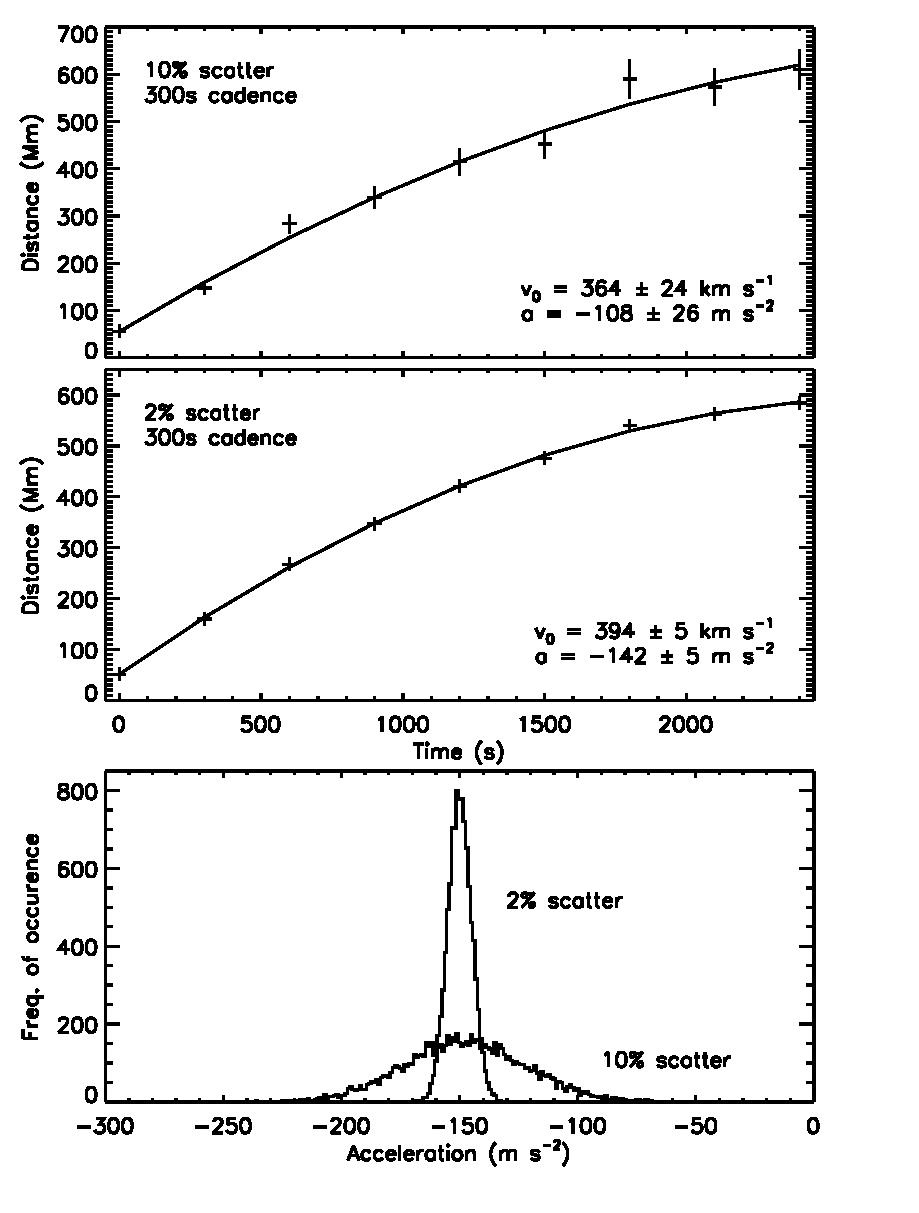
\includegraphics[width = 0.45\textwidth]{images/noise_hist_jpb.eps}
\caption{Simulated distance-time measurements with 3$\sigma$ scatters of $\pm$\,10\% (\emph{top}), and $\pm$\,2\% (\emph{middle}) of the model value, at a fixed cadence of $300\,s$, and the resulting quadratic fit and $v_0$ and $a$ parameters. The reduced scatter increases the precision for obtaining the true kinematics, as demonstrated by the different distributions of derived acceleration fit parameters (\emph{bottom}).}
\label{noise_hist_weight}
\end{center}
\end{figure}

\begin{figure}[!t]
\begin{center}
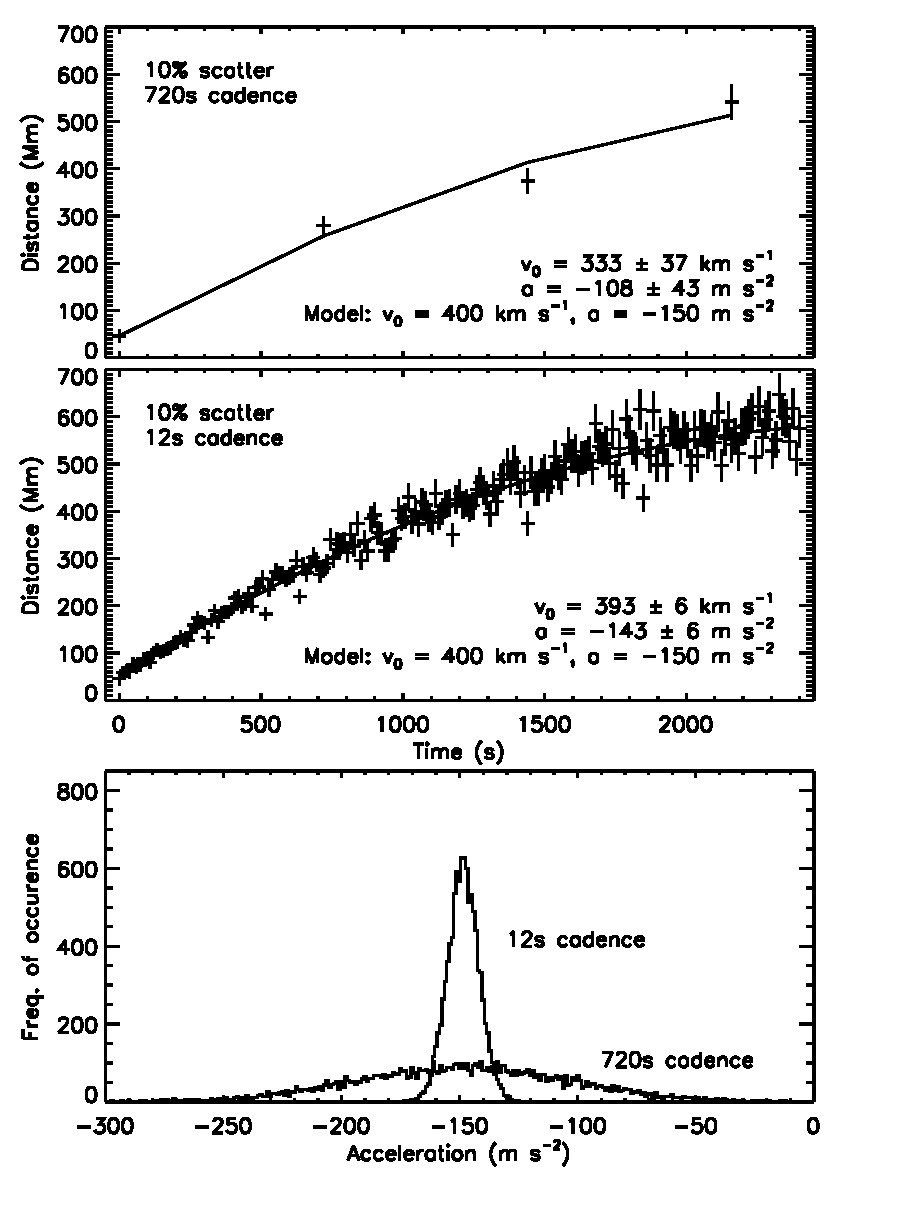
\includegraphics[width = 0.45\textwidth]{images/cad_hist_jpb.eps}
\caption{Simulated distance-time measurements for sampling cadences of $720\,s$ (EIT; \emph{top}) and $12\,s$ (AIA; \emph{middle}), at a fixed scatter of $\pm\,10\%$, and the resulting quadratic fit and $v_0$ and $a$ parameters. The increased cadence offers better precision for obtaining the true kinematics, as demonstrated by the different distributions of derived acceleration fit parameters. (\emph{bottom}).}
\label{cad_hist_weight}
\end{center}
\end{figure}

\begin{figure}[!b]
\begin{center}
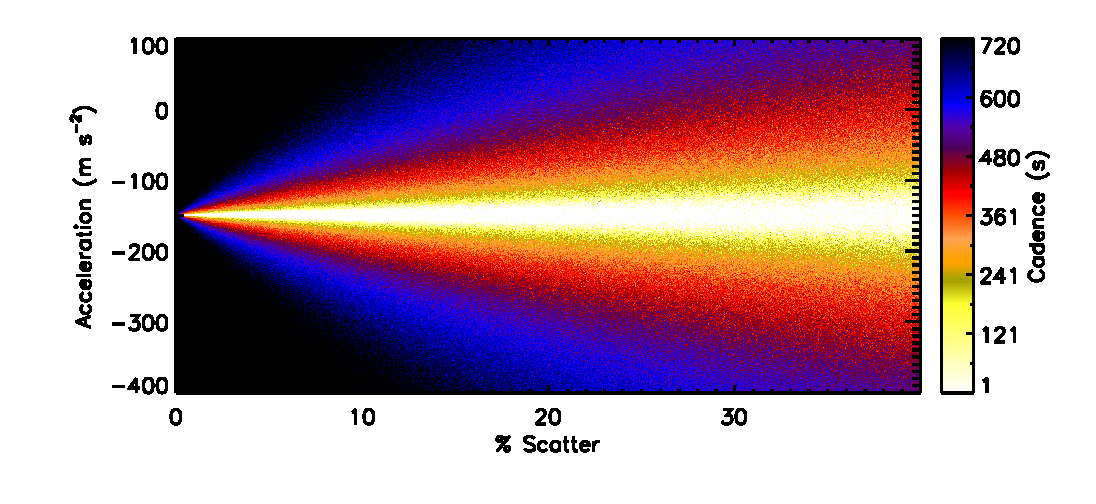
\includegraphics[scale=0.53, trim=20 10 0 20]{images/fig_noise_cad.eps}
\caption{Simulation of the derived accelerations from the model fits to Equation~\ref{eqn:const_a} (with examples shown in Figures~\ref{noise_hist_weight} and \ref{cad_hist_weight}), for scatters of 0\,--\,40\% and cadences of 1\,--\,720\,s. As shown, a decrease in both the data scatter and the cadence time improves the chances of obtaining the correct acceleration value, being $-150$\,m\,s$^{-2}$ in this model coronal wave case.}
\label{noise_test_image}
\end{center}
\end{figure}

\begin{figure*}[!t]
\centering
\subfigure{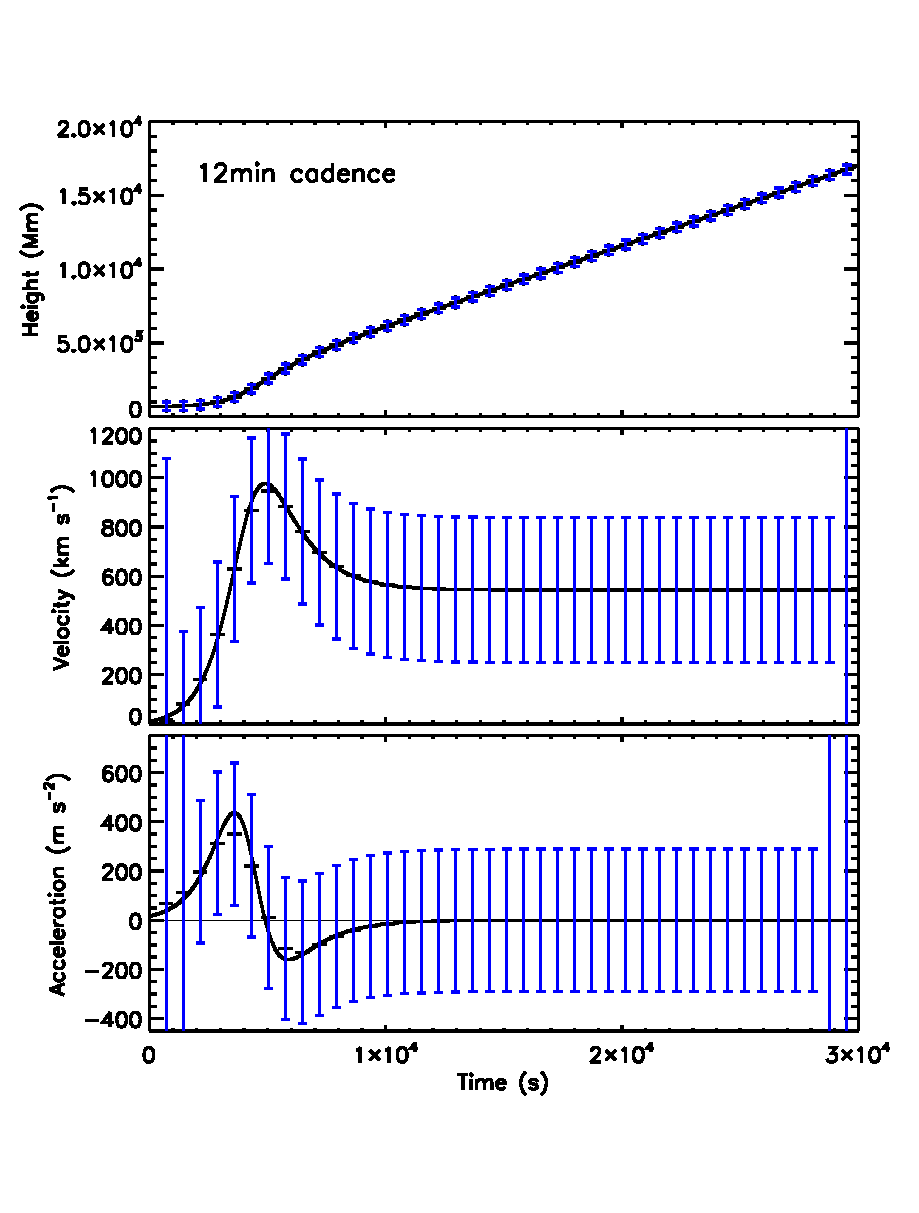
\includegraphics[scale=0.5, trim=0 55 0 50]{images/fig_cadence_hva_12min.eps}}
\subfigure{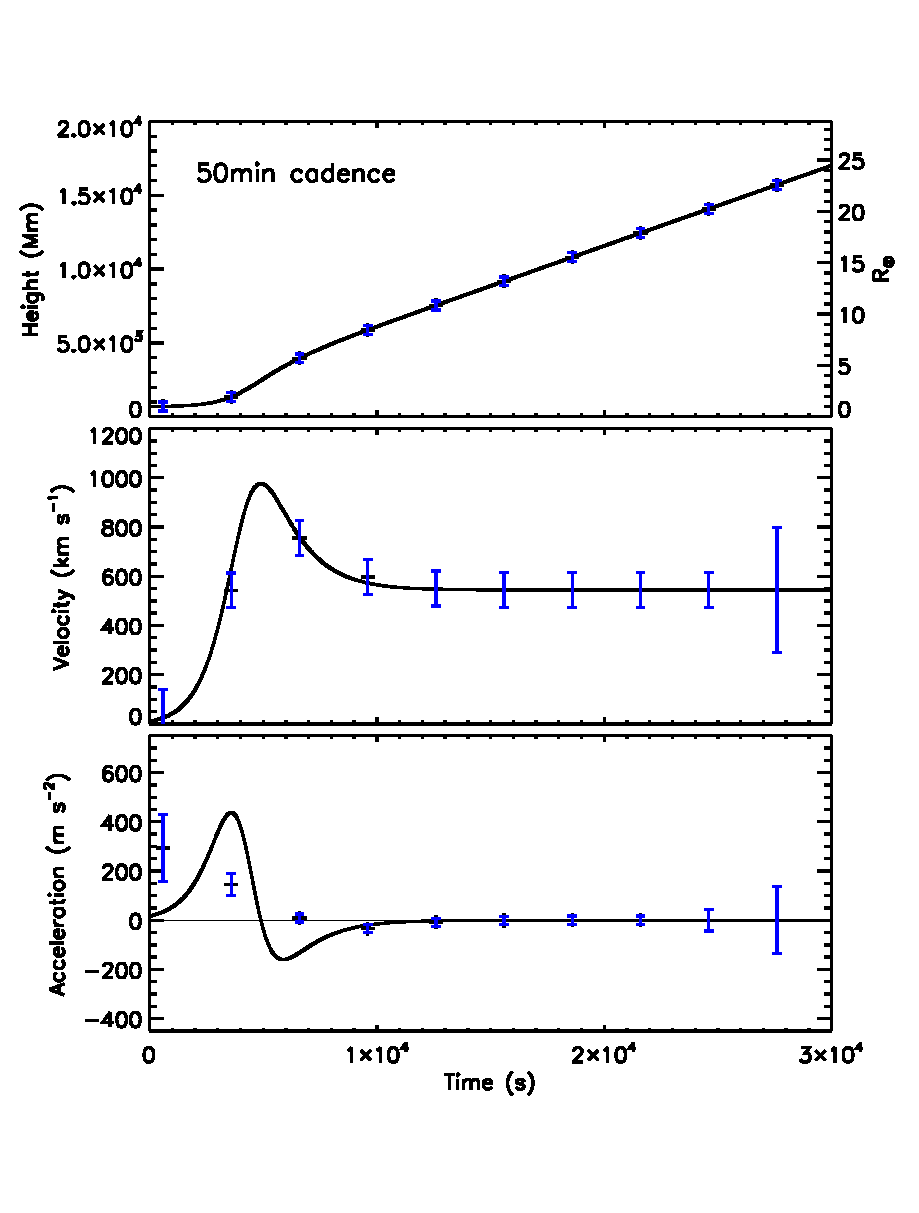
\includegraphics[scale=0.5, trim=0 55 0 50]{images/fig_cadence_hva_50min.eps}}
\subfigure{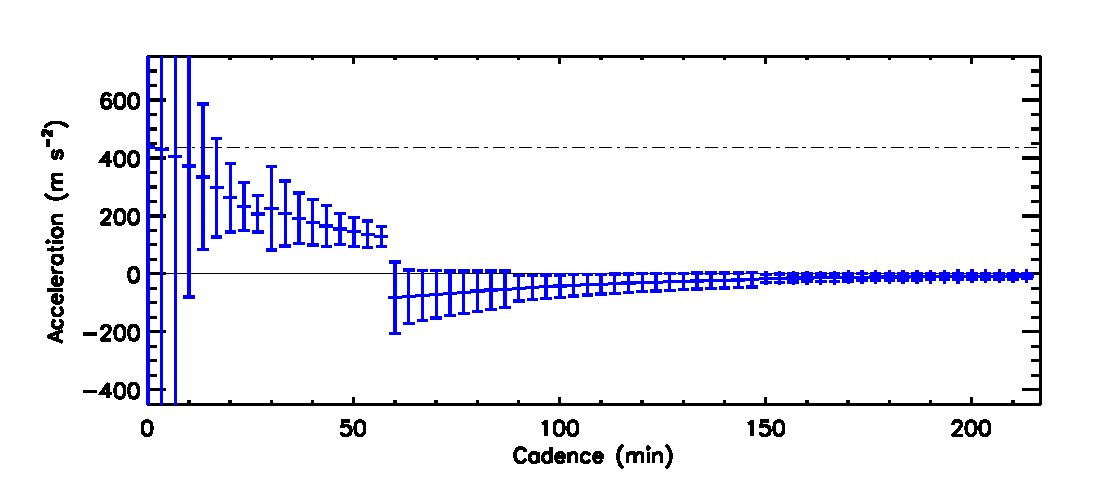
\includegraphics[scale=0.5, trim=0 20 0 25]{images/fig_cadence_1.eps}}
\caption{A demonstration of the effects of cadence on the error propagation according to the 3-point Lagrangian interpolation. A kinematic model for a CME with non-constant acceleration peaking at $437\,m\,s^{-2}$ is tested for varying cadences, without any scatter. The top left panels show the height, velocity and acceleration plots for data sampled at 12\,minute cadence. The top right panels show similar for 50\,minute cadence. Note how the errorbars of the higher cadence measurements are counter-intuitively larger than the lower cadence measurements, even though the higher sampling rate better reveals the true kinematic trend. The bottom panel shows the derived peak acceleration against cadence, where the dot-dashed line indicates the true value of $437\,m\,s^{-2}$. The errorbars are shown to reduce in magnitude (implying greater precision) even though the derived acceleration at lower cadence is less accurate.}
\label{fig_cadence_hva}
\end{figure*}

As an example of the effect of measurement scatter in the data, we first simulate a simple height-time profile of a CME that propagates according to the quadratic equation
\begin{equation}
\label{eqn:const_a}
r(t) = r_0 + v_0 t + \frac{1}{2}a t^2
\end{equation}
where $r_0=60\,Mm$ is the initial height, $v_0=300\,km\,s^{-1}$ is the initial velocity, and $a=2\,m\,s^{-2}$ is the acceleration of the CME. Measurement scatter is applied to the height-time points via a normally-distributed random number generator with a standard deviation of 10\% of the model height at each time-step. An `extreme case' errorbar on each measurement is determined by its distance from the true height-time profile, to represent a scenario wherein all measurement uncertainties just manage to overlap the true profile. Various instances of randomised measurement scatter result in erroneous trends in the velocity and acceleration profiles, even with the proper error treatment prescribed by the 3-point Lagrangian interpolation technique, and even in this simple case of constant acceleration. Two examples are shown in the left and right of Figure~\ref{sim_vels_thesis} where completely opposing acceleration trends are determined for different samplings of the same height-time dataset, indicating that the nature of the scatter in the samples is not satisfactorily reflected in the derived kinematics and their associated errorbars. At the very least the kinematic uncertainties should be expected to overlap the truth in each plot so that it remains a valid solution. A possible assurance, even in the case of low-cadence samplings (or very fast events), is that instead of trusting the endpoints, they simply be removed. Figure~\ref{sim_vels_thesis} would then show three datapoints for velocity and one datapoint for acceleration, that would reduce the biased trends and imply a constant acceleration close to the true value. However, when dealing with low-number samples, it would be better not to have to remove datapoints.


The effects of scatter on the distance-time measurements of a coronal wave were also examined, demonstrated here for the case of a constant acceleration event. The wave motion is modeled by Equation~\ref{eqn:const_a}, where $r_0\,=\,50\,Mm$ is the initial distance of the wave from the source, $v_0\,=\,400\,km\,s^{-1}$ is the initial velocity of the wave, and $a\,=\,-150\,m\,s^{-2}$ is the acceleration of the wave. Figure~\ref{noise_hist_weight} shows the derived kinematics for the simulated distance-time measurements with random scatter added, shown here for 3$\sigma$ limits of 10\% (top panel) and 2\% (middle panel). Model errorbars are applied, appropriate to the measurement scatter. A second-order polynomial (quadratic) is then fit to each dataset to test how the scatter affects the precision of the derived kinematics, even in this idealized case of knowing the underlying form of the data. The increased scatter acts to smooth out the true kinematics, as demonstrated by the different distributions of derived accelerations (bottom panel).


\subsection{Effect of Sampling Cadence on Deriving Kinematics}
\label{subsect:cadence}

As an example of the effect of cadence, we first simulate again the constant-acceleration profile of a coronal wave (as in Equation~\ref{eqn:const_a} and Figure~\ref{noise_hist_weight}). The simulated distances were sampled at cadences akin to the instruments SOHO/EIT (12\,mins) and SDO/AIA (12\,secs), at a fixed $3\sigma$ scatter of 10\% of the model distance. Model errorbars are again applied, as appropriate. Figure~\ref{cad_hist_weight} shows examples of these, with a quadratic fit to the sample measurements to test the effect on the derived kinematics. It is clear that the higher-cadence data best resolves the true kinematic profile, providing an accurate estimation of the wave velocity and acceleration. These results are consistent with the observations made by both \citet{2008ApJ...680L..81L} and \citet{2009ApJ...707..503M} and show that the effects of image cadence must be accounted for when determining the kinematics of a coronal wave.

In Figure~\ref{noise_test_image} the combined effects of measurement scatter and sampling cadence are simulated for the model coronal wave case. The figure shows the result of plotting the distribution of acceleration fit parameters against all variations of scatter from $0$\,--\,$40\%$, at all variations of cadence from $1$\,--$720\,s$. Essentially the plots of the bottom panels of Figures~\ref{noise_hist_weight} and \ref{cad_hist_weight} represent slices through the corresponding locations of Figure~\ref{noise_test_image}. This demonstrates that the reduction of measurement scatter and increase of sampling cadence together are required to improve the accuracy of the derived kinematics.

We next simulate a non-constant acceleration profile for a typical fast CME via the following equations (where the constant $s$ is just a scaling factor):
\begin{eqnarray}
h(t)\,=&\,\sqrt{2s}\,t\tan^{-1}\left(\frac{e^{t/2s}}{\sqrt{2s}}\right) \\
v(t)\,=&\,\sqrt{2s}\tan^{-1}\left(\frac{e^{t/2s}}{\sqrt{2s}}\right)+\frac{e^{t/2s}t}{e^{t/s}+2s} \\
a(t)\,=&\,\frac{e^{t/2s}\left(2s\left(t+4s\right)-e^{t/s}\left(t-4s\right)\right)}{2s\left(e^{t/s}+2s\right)^2}
\label{eqn:nonconst_a}
\end{eqnarray}
The acceleration profile exhibits an initial peak followed by a deceleration and then leveling to zero. This is akin to a general impulsive CME that undergoes an initial high-acceleration eruptive phase, and then decelerates to match the solar wind speed during its propagation phase. A model CME height-time profile is generated, enabling synthetic observation samples to be taken at different cadences. 

We investigate the effect of the cadence of the observations on the derivation of the kinematics and associated errorbars using the standard 3-point Lagrangian interpolation. In the first instance fixed errorbars of $\pm\,300\,Mm$ are applied to the height-time measurements, without any scatter. This is useful to simply test the effects of the cadence on the derived velocity and acceleration profiles and their associated errors. The top left and right plots of Figure~\ref{fig_cadence_hva} show the model height-time, velocity and acceleration profiles sampled at cadences of 12 and 50\,minutes respectively. As the cadence is reduced, i.e., the time interval between observations is increased, the errorbars become smaller due to the inverse dependence of the Lagrangian error terms on the time between the datapoints $\Delta t^{-2}$ (see Equation~\ref{vel_err}). However, reducing the cadence reduces the resolution at which the acceleration peak is detectable, and so the acceleration profile is less well characterized. Conversely, the errorbars become erroneously large for very high-cadence measurements, even though the measurements better reveal the true trends of the kinematic profiles, as demonstrated in the bottom panel of Figure~\ref{fig_cadence_hva}. This fundamentally implies that the errorbars do not truly reflect the uncertainty on the data at a given cadence, and are in fact redundant for these cases.

%As a result, two distinct kinematic forms were simulated here: a quadratic model and a power--law model. Both of these models are typically used to determine the kinematics of these disturbances and have been used extensively in previous work \citep[e.g.,][]{2008ApJ...680L..81L,2008ApJ...681L.113V,2004A&A...418.1101W,2011ApJ...739...89M}. The quadratic model takes the form of Equation~\ref{eqn:const_a} assuming the wave moves with constant acceleration. The power-law fit may be used to identify variable acceleration of the form:
%\begin{equation}
%r(t) = c(t - t_0)^{\gamma}
%\end{equation}
%where $c$ is a constant, $t_0$ is the start time, and $\gamma$ is the exponent.


It is clear therefore, that the variation in both scatter and imaging cadence can strongly influence the derived kinematics of a CME or coronal wave, and the commonly used 3-point Lagrangian technique does not return useful estimates of the associated uncertainty. Furthermore, the quantification of uncertainty on the physical measurements themselves is extremely non-trivial. This is due to the effect of `unknown unknowns' throughout the analysis, making a robust error estimate practically impossible. This is especially true for automated routines designed to detect faint and transient phenomena such as CMEs and coronal waves, being prone therefore to unpredictable biases. However, it is possible to use other techniques in an effort to overcome these issues, and produce a more statistically sound method for dealing with these types of measurements.


\section{Bootstrapping: a resampling method}
\label{sect:bootstrapping}

\begin{figure}
\begin{center}
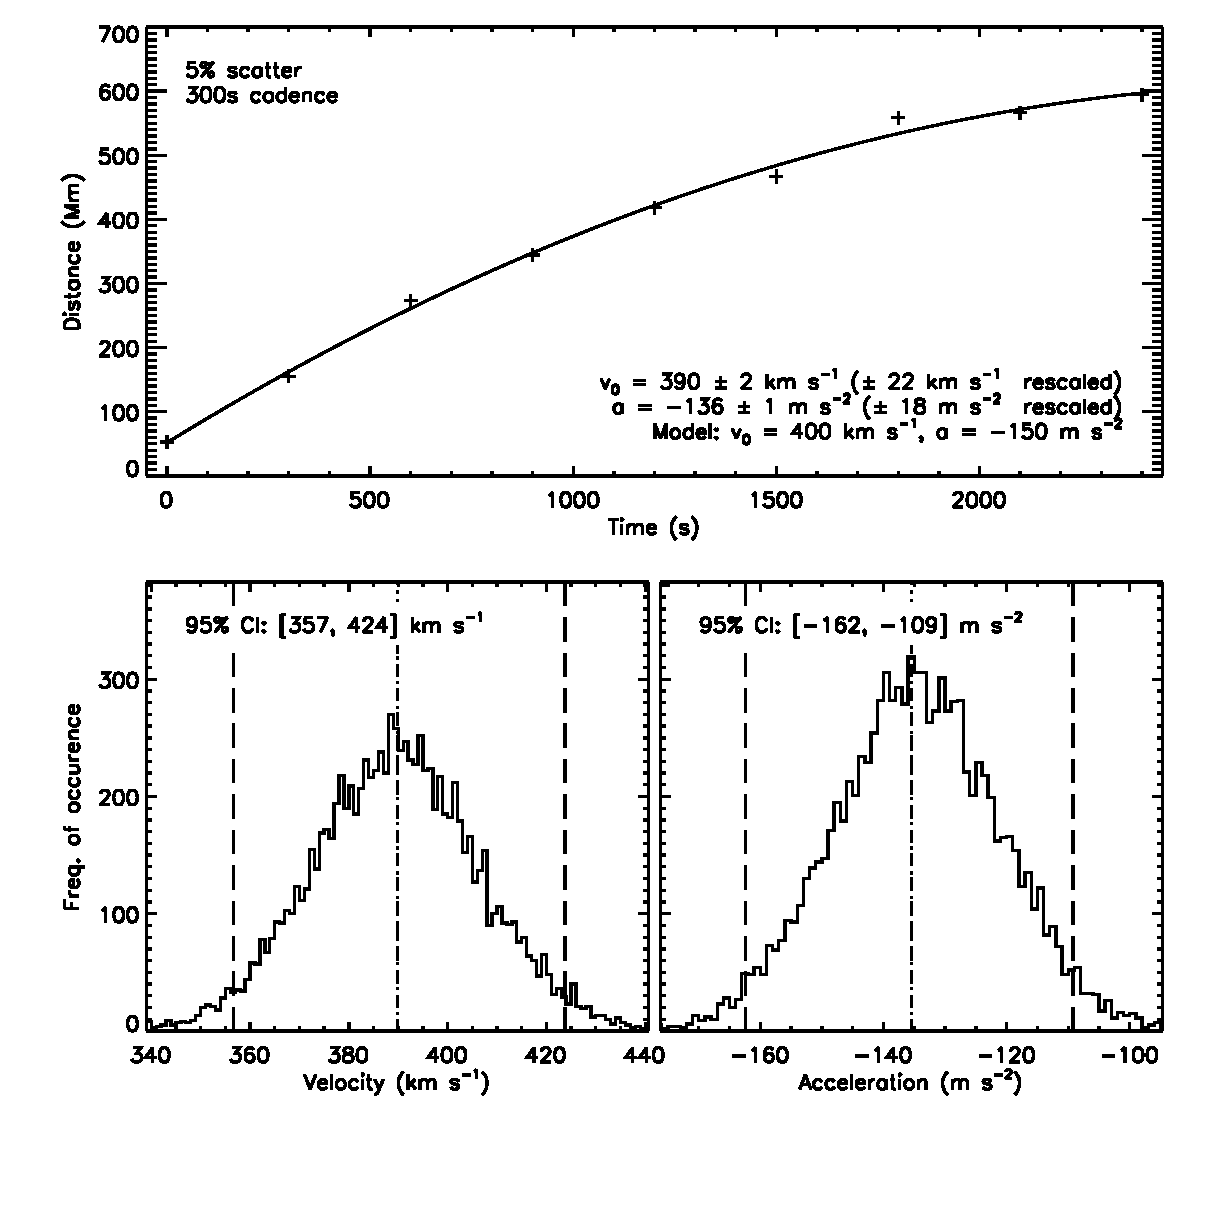
\includegraphics[scale=0.45, trim=20 50 0 0, clip=true]{images/cad_boot_weight_jpb.eps}
\caption{Top panel shows the initial fit of Equation~\ref{eqn:const_a} to simulated coronal wave distance-time measurements, with 5\% scatter and $300\,s$ cadence. Errorbars of $\pm1.1\,Mm$ are assigned to the measurements, based on the 1.5 arcsec resolution of the imager. The fit parameters are quoted with $1\sigma$ uncertainties, with the rescaled uncertainties shown in brackets. The bottom panels show histograms of the initial velocity and acceleration values derived using the bootstrapping technique. The mean and 95\% confidence interval are indicated by the dot-dashed and dashed lines respectively. Bootstrapping provides a distribution of fitting parameters that is unattainable via a standard single-fit to data when `unknown unknowns' exist as a source of uncertainty.}
\label{cad_boot_weight}
\end{center}
\end{figure}

When trying to determine an estimator for a particular parameter of interest and subsequently evaluate the accuracy of that estimator, a small sample size is immediately limiting. Therefore, in order to approximate the behavior of the true distribution, techniques based on resampling methods have been developed. These work by resampling the data enough times to generate a maximum likelihood estimator of the distribution. Bootstrapping, first introduced by \citet{Efron:1979p1831} and more recently described in, e.g., \citet{1994.book.Efron} and \citet{Chernick1999}, is one such technique, that may be formally defined as follows: Given a random sample of $n$ independent identically distributed vectors $\vec{x} = \left( x_1, x_2, ..., x_n \right)$ from an unknown probability distribution function $\vec{F}$ and a real-valued estimator $\hat{\theta} = s \left( \vec{x} \right)$, a procedure (the bootstrap) to assess the accuracy of $\hat{\theta}$ is defined in terms of the empirical distribution function $\hat{\vec{F}}$, which is the maximum likelihood estimator of the distribution for the observations when no parametric assumptions are made. Otherwise stated, a bootstrap sample $\vec{x}^* = \left( x_1^*, x_2^*, ..., x_n^* \right)$ is generated by randomly sampling with replacement from the population of $n$ objects, giving a resampled version of $\vec{x}$. The bootstrap algorithm then works by drawing many independent bootstrap samples, to estimate the standard error of $\hat{\theta}$ from the observed data $\vec{x}$.

In the cases of CME and coronal wave observations, bootstrapping techniques can prove very useful for determining the confidence on the derived kinematic or model parameters. The implementation of the bootstrap is as follows:
\begin{enumerate}
\item An initial fit to the data $y$ is obtained, yielding the model fit $\hat{y}$ with parameters $\vec{p}$.
\item The residuals of the fit are calculated: $\epsilon = y - \hat{y}$.
\item The residuals are randomly resampled with replacement to give $\epsilon^*$.
\item The model is then fit to a new data vector $y^* = y + \epsilon^*$ and the parameters $\vec{p}^*$ stored.
\item Steps 3--4 are repeated many times (e.g. 10,000).
\item Confidence intervals on the parameters are determined from the resulting distributions.
\end{enumerate}
This technique was used to fit a quadratic model, first to the simulated coronal wave moving with constant acceleration (Equation~\ref{eqn:const_a}), and second to the simulated CME moving with non-constant acceleration (Equation~\ref{eqn:nonconst_a}). In the case of the wave, the initial fit to the measurements and the bootstrapped distributions of initial velocity and acceleration values are shown in Figure~\ref{cad_boot_weight}. Bootstrapping in this manner allows the determination of confidence intervals on the fit parameters. This is taken from the 100$\alpha$th and 100$\left(1-\alpha\right)$th percentiles of the distribution (giving a 95\% confidence interval when $\alpha=.025$). Since there exist `unknown unknowns' that can affect the measurement scatter, the only uncertainty that can be confidently attributed to the measurements is that which is due to the resolution limit of the data and similar quantifiable sources of uncertainty. Therefore, in an effort to avoid assigning incorrect uncertainties that will undermine the interpretation of any subsequent model-fit, the scatter of the data instead may be investigated via resampling methods.

For the simulated measurements in Figure~\ref{cad_boot_weight}, the datapoints were assigned errorbars of $\pm1.1\,Mm$, based on the 1.5 arcsec resolution of AIA \citep{2012SoPh..275...17L}, representing the lower limit of quantifiable uncertainty. If, as in this simulated coronal wave case, it may be assumed that the model should give an appropriate fit to the data, and the measurement uncertainties are known to be too small (or alternatively too large), then the output uncertainties on the fit parameters can be rescaled accordingly, as per the following equation:
\begin{equation}
\sigma'^2 = \sigma^2 \times \chi^2 / \nu
\end{equation}
where $\nu$ is the number of degrees of freedom in the fit \citep[see, for example,][]{2003drea.book.....B}. The rescaled uncertainties for this case are quoted in the top panel of Figure~\ref{cad_boot_weight}. However, since in truth we do not know the exact kinematic form a CME or coronal wave should take, nor the true uncertainty due to `unknown unknowns', we cannot make such assumptions in our treatment of the real-data measurements. Therefore the power of a bootstrapping technique is clear, allowing an appropriate confidence interval to be assigned to the fit parameters. For the simulated measurements in Figure~\ref{cad_boot_weight}, it is seen that the bootstrapped distributions for the initial velocity and acceleration do contain the true model values, and also have a range akin to the rescaled uncertainties of the single fit (i.e., likening the 95\% confidence intervals to $2\sigma$ uncertainty ranges, which are approximately double the rescaled $1\sigma$ uncertainty ranges of the single fit).

\begin{figure}[t]
\centering
\subfigure{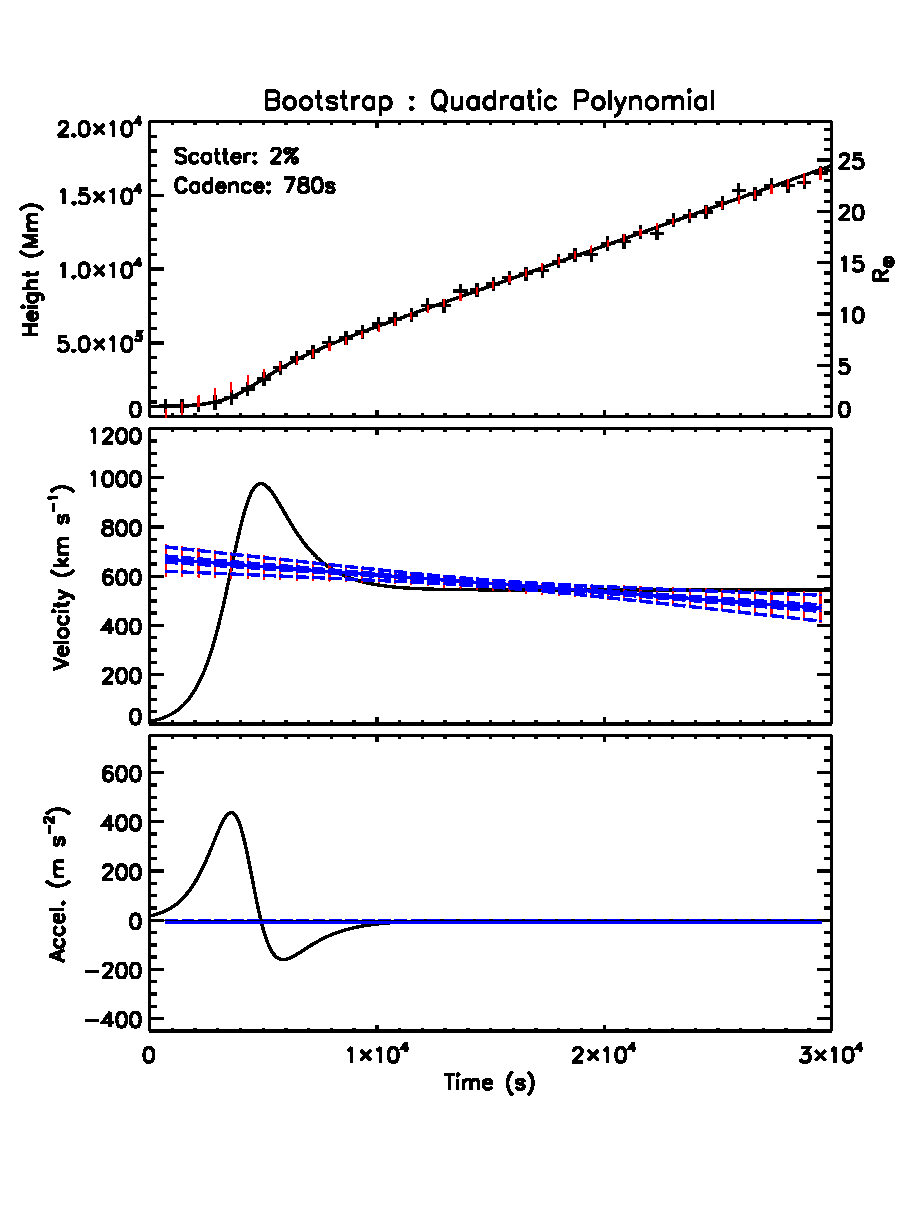
\includegraphics[scale=0.6, trim=0 80 0 30]{images/fig_bootstrap_quadratic.eps}}
\subfigure{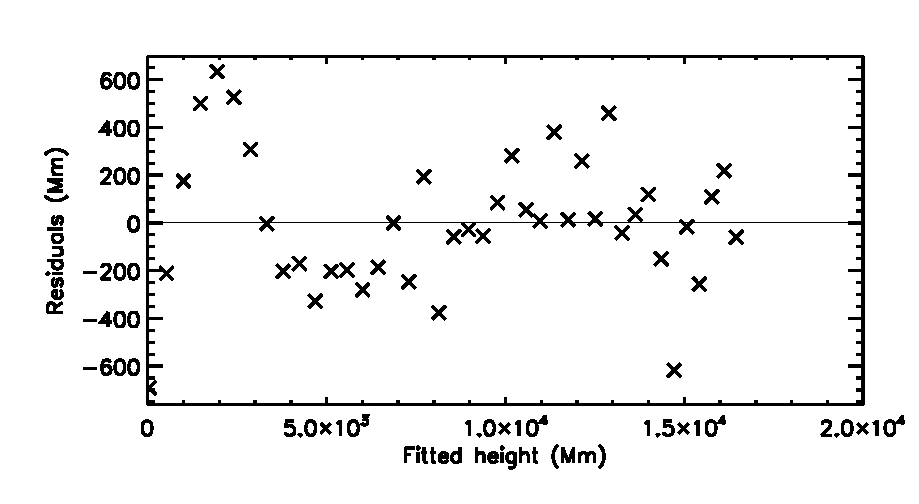
\includegraphics[scale=0.6, trim=0 20 0 0]{images/fig_residuals_quadratic.eps}}
\caption{The bootstrapped second order polynomial fit to simulated CME height-time measurements, with 2\% scatter and 780$\,s$ cadence. The panels from top to bottom show the height, velocity, and acceleration plots, and the residuals of the initial fitted height. The red points show the resampled residuals with replacement, and the blue dashed lines are the median, interquartiles range, and upper and lower fences on the bootstrapped fit. The quadratic form tends to smooth out the non-constant acceleration profile, as revealed by the trend in the residuals, indicating that the fit is not appropriate for the measurements.}
\label{fig_quadratic}
\end{figure}

\begin{figure}[t]
\centering
\subfigure{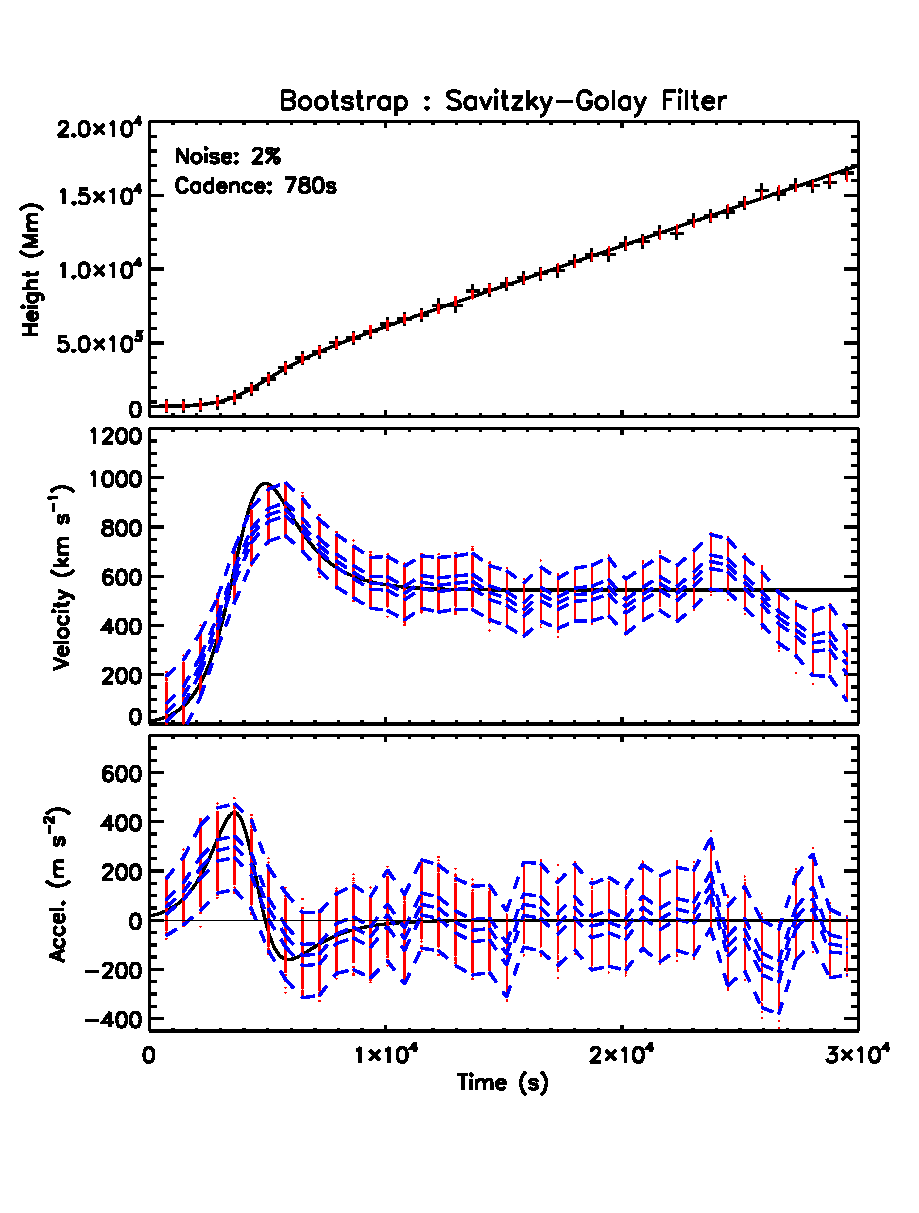
\includegraphics[scale=0.6, trim=0 80 0 30]{images/fig_bootstrap_savgol.eps}}
\subfigure{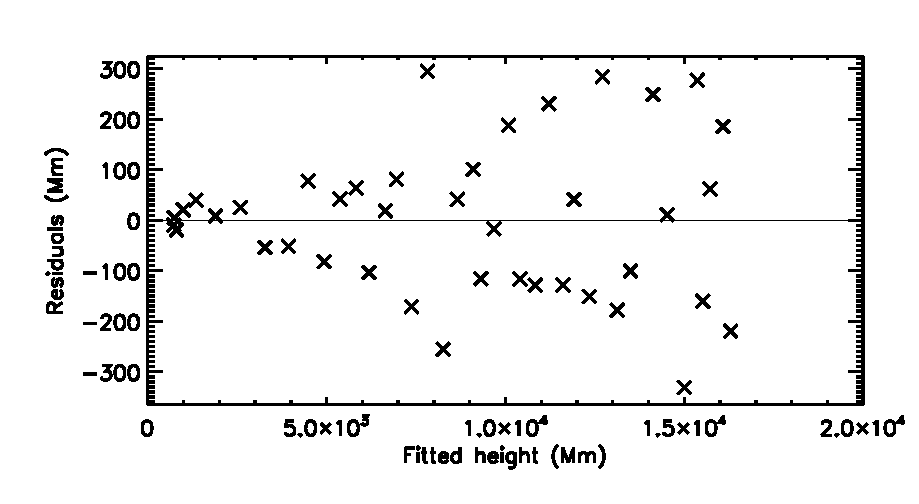
\includegraphics[scale=0.6, trim=0 20 0 0]{images/fig_residuals_savgol.eps}}
\caption{The bootstrapped Savitzky-Golay filter method applied to the simulated CME height-time measurements as in Figure~\ref{fig_quadratic}. This manner of piecewise fit smooths the measurements by fitting a polynomial to the 3 neighboring points either side of each datapoint, and is successful in revealing the non-constant acceleration profile. The randomly scattered residuals also indicate its appropriateness.}
\label{fig_savgol}
\end{figure}

Bootstrapping of a model cannot be applied blindly, as we will demonstrate for a simple case of fitting the same constant acceleration form of Equation~\ref{eqn:const_a} to the non-constant acceleration of Equation~\ref{eqn:nonconst_a}. Figure~\ref{fig_quadratic} shows the associated model CME profile, sampled at 780$\,s$ cadence with 2\% scatter. The red points show the resulting distributions of points after the residuals are resampled with replacement. Thus a distribution of velocity and acceleration values are derived, with the corresponding median, interquartile range, and upper and lower fences overlaid in blue. The second-order model is not appropriate to the true non-constant acceleration profile, as revealed by the trend in the residuals of the initial fit (bottom panel of Figure~\ref{fig_quadratic}). So for any cases where possible non-constant acceleration profiles are to be revealed, the method for deriving the kinematics must be applied at an appropriate scale, and such that the residuals scatter randomly. Ideally a piecewise function should be used to characterize the different phases of motion. This is inspected in great detail by \citet{2008ApJ...674..586S} in an effort to model the early acceleration phase of erupting filaments involved in CMEs. They show that one functional form alone cannot describe the entire phase as well as a number of different functions can. Since we do not know the functional form that CME or coronal wave kinematics will have, we must rely on some form of numerical derivative for revealing possible trends. Since the issues with the 3-point Lagrangian have been highlighted in Section~\ref{sect:simul1}, we shall opt instead to implement the Savitzky-Golay filter \citep{Savitzky-Golay1964}. This is a form of local polynomial regression of chosen degree of smoothing polynomial, and of chosen order to produce smoothed first order, second order, etc., derivatives of the signal. The number of datapoints either side of the case point to be included in the filter is also specified. Therefore, in the case of CME and coronal wave distance-time measurements, the Savitzky-Golay filter is a better method for smoothing small-scale scatter while still revealing the true kinematic profiles. This is illustrated in Figure~\ref{fig_savgol} for the simulated non-constant acceleration profile, with the residuals resampled with replacement as per the bootstrapping technique described above and demonstrated in Figures~\ref{cad_boot_weight} and \ref{fig_quadratic}. For this case the neighboring 3 points to the left and right of each datapoint were considered. Since it is a form of ``moving window averaging", slight biases may be introduced at local maxima and minima where the function value can be reduced, but its implementation still proves more robust that the standard 3-point Lagrangian. Note that the residuals can be seen to scatter somewhat randomly, as desired (bottom panel of Figure~\ref{fig_savgol}). Also, for this case-study it is important to note how the scatter at the endpoints gives the impression of a decreasing velocity which the Savitzky-Golay filter faithfully reproduces even though we know it is not how the model is behaving. This is akin to how the intensity of a CME or coronal wave often lies too close to the background intensity at such distances, being lost to the noise and causing the measured profile to drop off. This alludes to considerations that must be made when dealing with automated systems of kinematic determination, whereby the algorithmic limitations can introduce systematic biases not accounted for in the derived kinematics and associated uncertainties. This is discussed further in the next section.


%\begin{figure}[t]
%\centering
%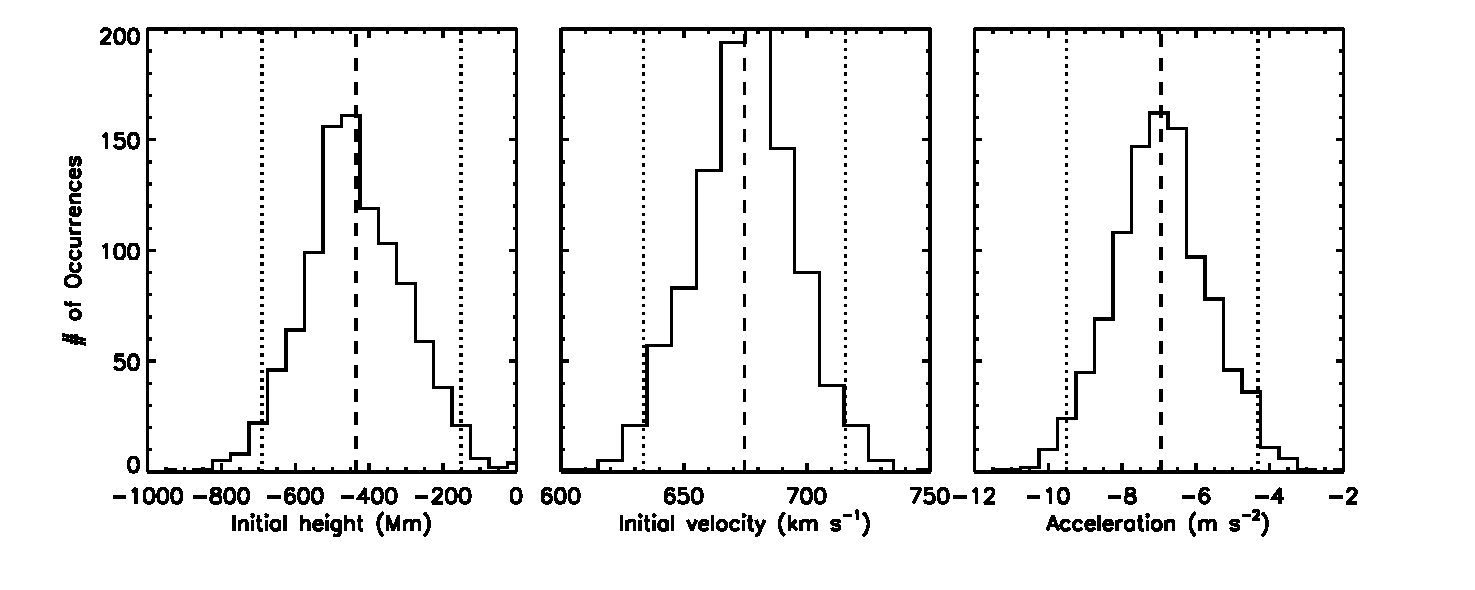
\includegraphics[width=0.5\textwidth, trim=25 0 0 0]{images/fig_bootstrap_quad_vals.pdf}\caption{Height: mean:       -435.53730
%sdev:        137.82235
%95\% CI:       -690.15195      -151.37066]
%Vel: mean:        674.65762
%sdev:        20.616389
%95\% CI:        633.63249       715.51399
%Accel: mean:       -6.9454313
%sdev:        1.3131190
%95\% CI:       -9.5047688      -4.3180026
%}
%\label{fig_bootstrap_quad_vals}
%\end{figure}

%\begin{figure}[t]
%\centering
%\subfigure{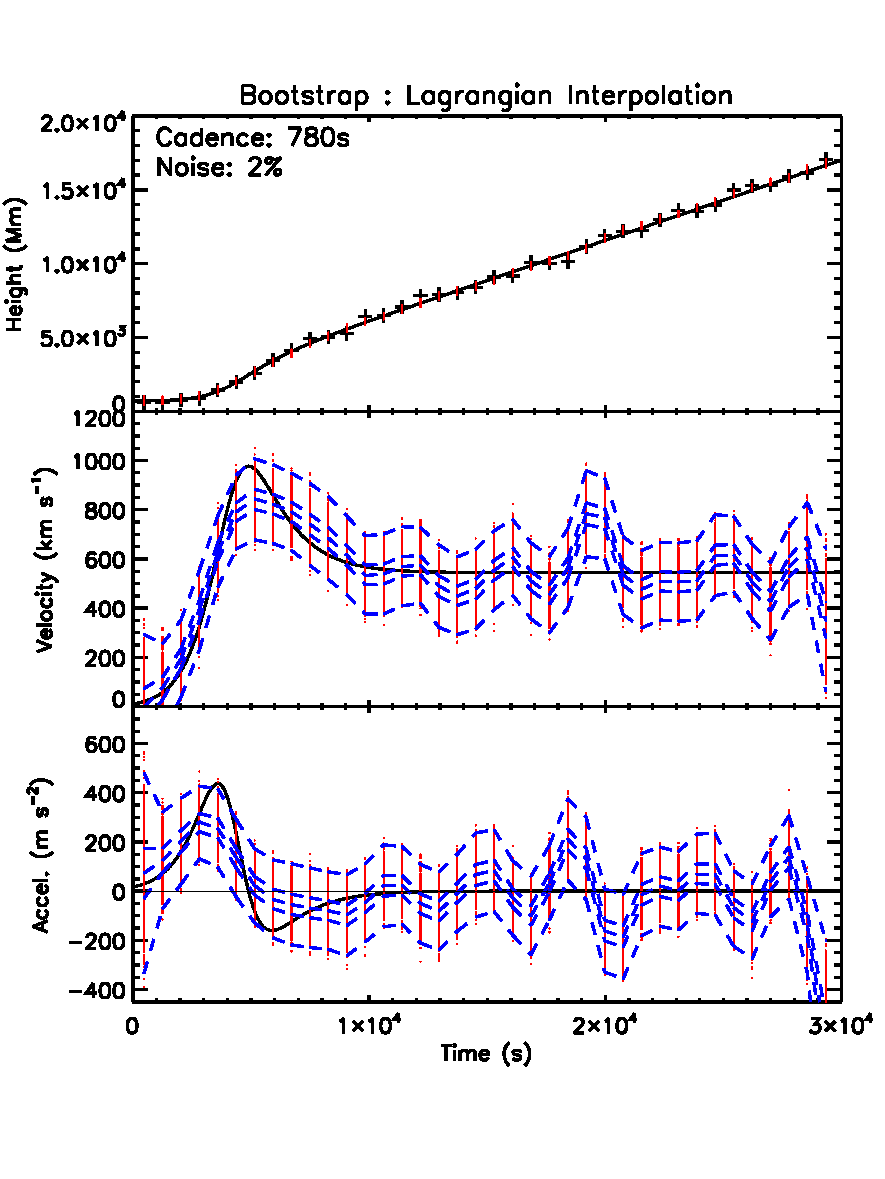
\includegraphics[scale=0.6, trim=0 80 0 30]{images/fig_bootstrap_lagrangian.pdf}}
%\subfigure{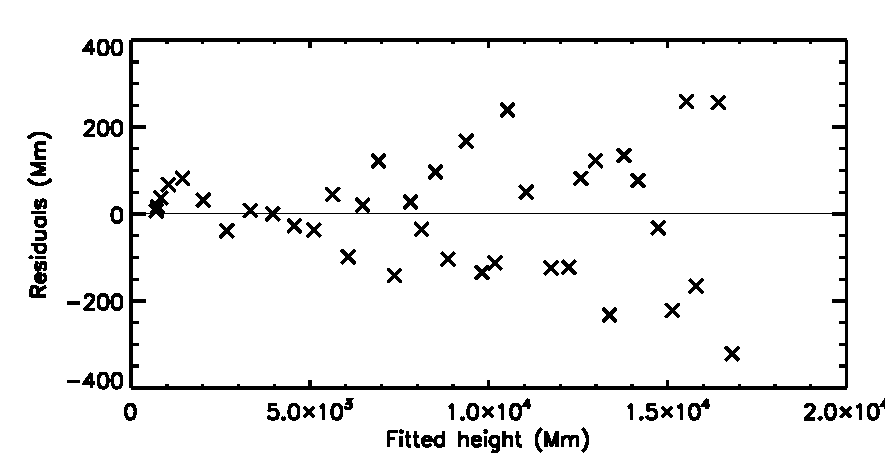
\includegraphics[scale=0.6, trim=0 20 0 0]{images/fig_residuals_lagrangian.pdf}}
%\caption{}
%\label{fig_lagrangian}
%\end{figure}

\section{Case Studies}
\label{sect:case_studies}

In this section some examples of real data are presented as case studies for deriving the CME and coronal wave kinematics in light of the discussion of the previous sections. %The newly developed CORIMP and CorPITA catalogues are used to detect and measure the distance-time profiles of CMEs and coronal waves in such a manner as to allow a determination of the ranges of speeds across the expanding phenomena as they propagate in time. They are inspected separately as follows.

\subsection{CME Kinematics}
\label{subsect:corimp}


First we shall revisit a CME studied by \citet{2009A&A...495..325B}, that was observed by SOHO/LASCO on 2000 January 2. In that study, the CME front edge was detected via multiscale methods and characterized with an ellipse-fit that was used to track changes to the CME front over time. The apex of the fit (furthest distance from Sun-centre) in each frame was measured, and a height-time profile produced. This allowed an investigation into the kinematics of the event, derived using the 3-point Lagrangian method and associated error propagation formulation. However, as has been outlined in the preceding sections, this formulation is somewhat redundant for such a small sample size, and so a new method is applied to test the validity of the analysis.

The method chosen, and deemed most appropriate from our investigations in this paper, is that of the Savitzky-Golay filter and bootstrapping technique. The filter width is set at 6 datapoints (3 neighbouring points either side of the point in question). The top panel of Figure~\ref{fig_savgol_CME} shows the height-time plot of the CME (the plus symbols), the resampled residuals (in red) after applying the Savitzky-Golay filter, and corresponding median, interquartile range, and upper and lower fences on the bootstrapped data (blue lines). The middle and bottom panels show the derived velocity and acceleration profiles. An important point to note is that a priori knowledge about such events and the manner in which they are tracked, must be called upon when interpreting the derived kinematic profiles. For CMEs, the outer edge of the field-of-view is less reliable due to increased noise as the CME intensity falls-off, and also the overlap between coronagraphs can cause discrepancies in the derived kinematics. For this example, there appears to be a decrease in velocity, and negative acceleration, at the outer edge of C3, but by inspecting the resampled height-time measurements this may be deemed an artifact of the smoothing by the Savitzky-Golay filter when dealing with the scatter on the endpoints - an ongoing issue for small datasets. This strongly indicates the need for improved CME observations, through increased imager cadences and greater field-of-view coverage, but otherwise a spread of measurements across the full span of CMEs in current observations should be considered.


\begin{figure}
\centering
\includegraphics[scale=0.6, trim=0 40 0 30]{images/fit_kinscasestudy_CME.eps}
\caption{The bootstrapped Savitzky-Golay filter method applied to a CME event observed by SOHO/LASCO on 2000 January 2, revisited from \citet{2009A&A...495..325B}. The top panel shows the height-time measurements (\emph{plus symbols}), the resampled residuals (\emph{red points}), and the median (\emph{solid line}), interquartile range (\emph{inner dashed lines}), and upper and lower fences (\emph{outer dashed lines}). The middle and bottom panels show the corresponding velocity and acceleration profiles.}
\label{fig_savgol_CME}
\end{figure}

\begin{figure}[!t]
\centering
\subfigure{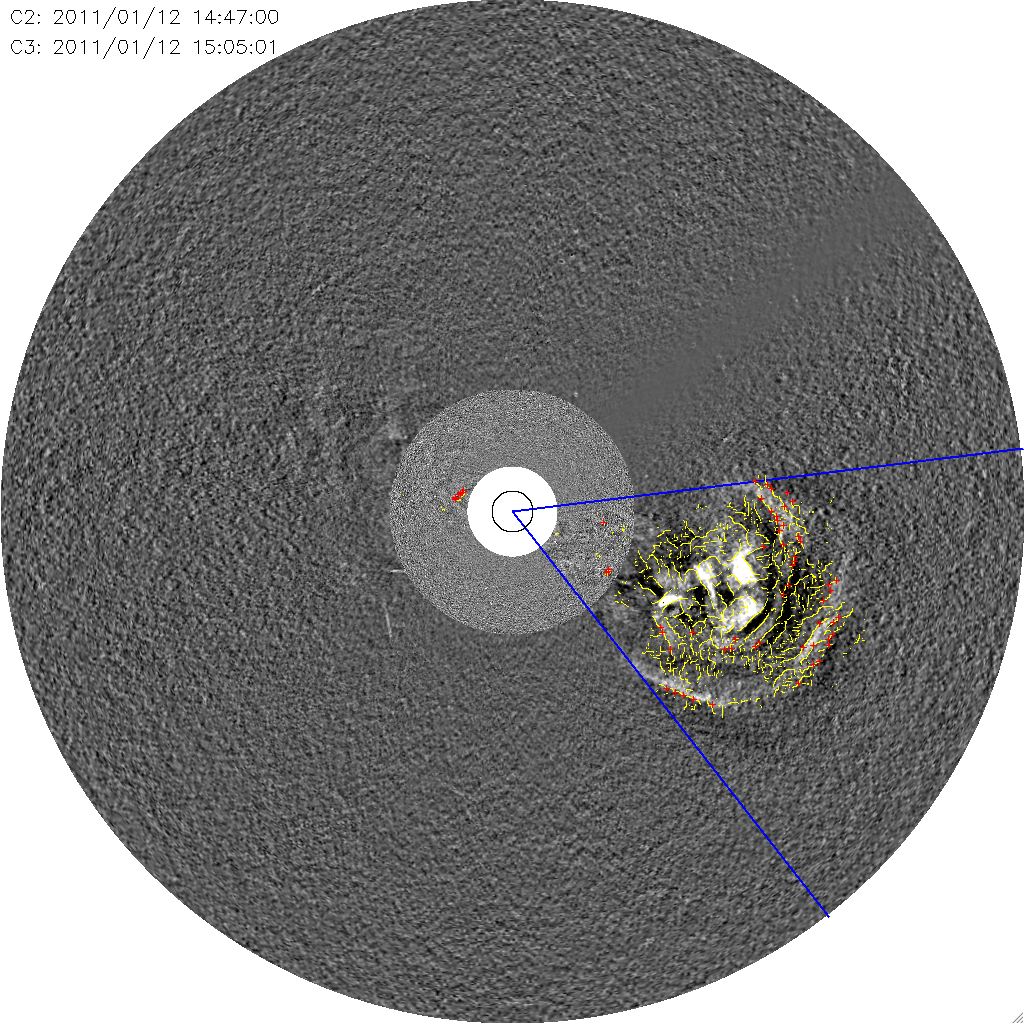
\includegraphics[scale=0.195, trim=0 90 150 0]{images/20110112_150501.png}}
\subfigure{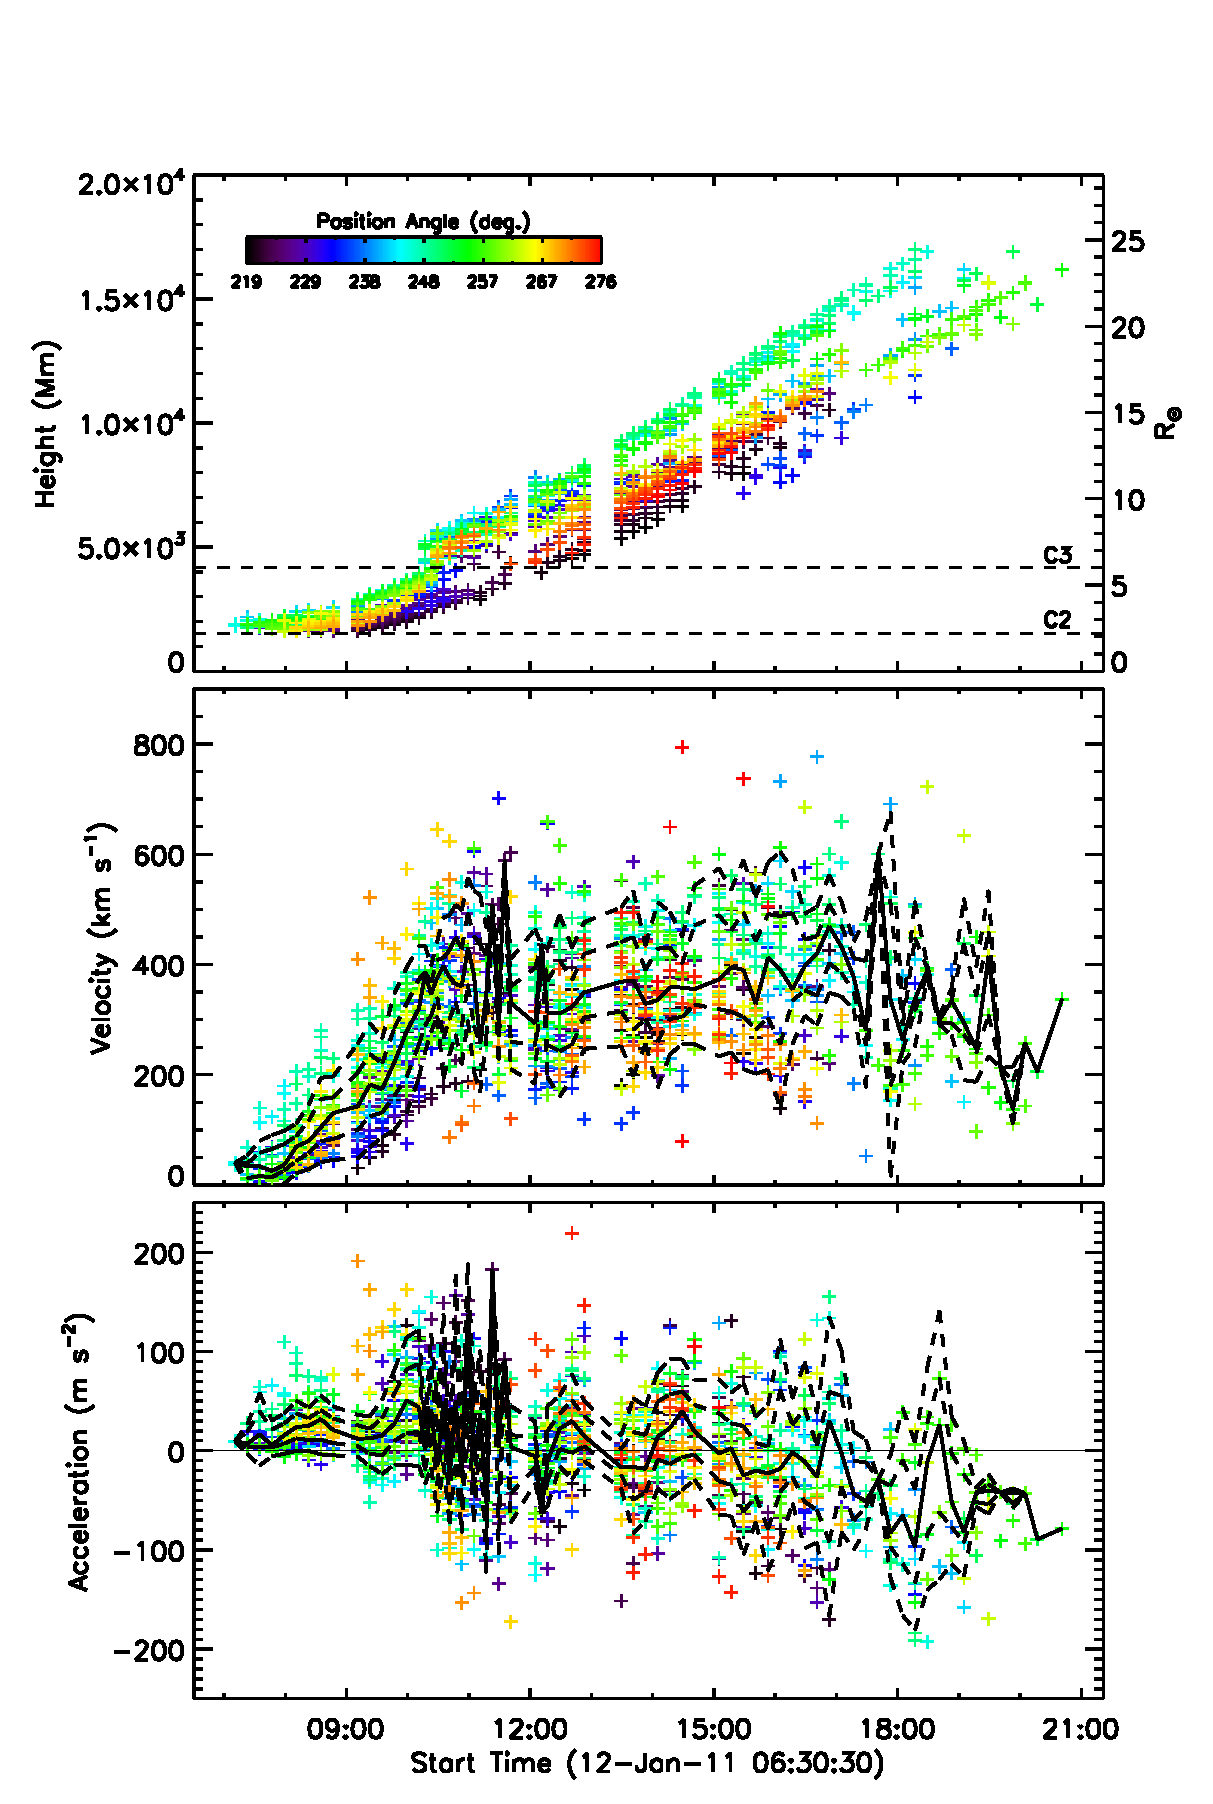
\includegraphics[scale=0.465, trim=15 20 0 60]{images/plot_kins_quartiles_20110112_savgol.eps}}
\caption{The Savitzky-Golay filter applied to the automated CORIMP CME detection and tracking of an event observed by SOHO/LASCO on 2011 January 12 (\emph{top image}). The detected CME structure is highlighted in yellow, and the outermost height measurements indicated in red. The top panel of the lower plot shows the height-time measurements across the angular range of the CME (indicated by the colourbar). The middle and bottom panels show the derived velocity and acceleration profiles, with the median (\emph{solid line}), interquartile range (\emph{inner dashed lines}) and upper and lower fences (\emph{outer dashed lines}) over-plotted.}
\label{fig_savgol_CME_CORIMP}
\end{figure}

%\begin{figure}
%\centering
%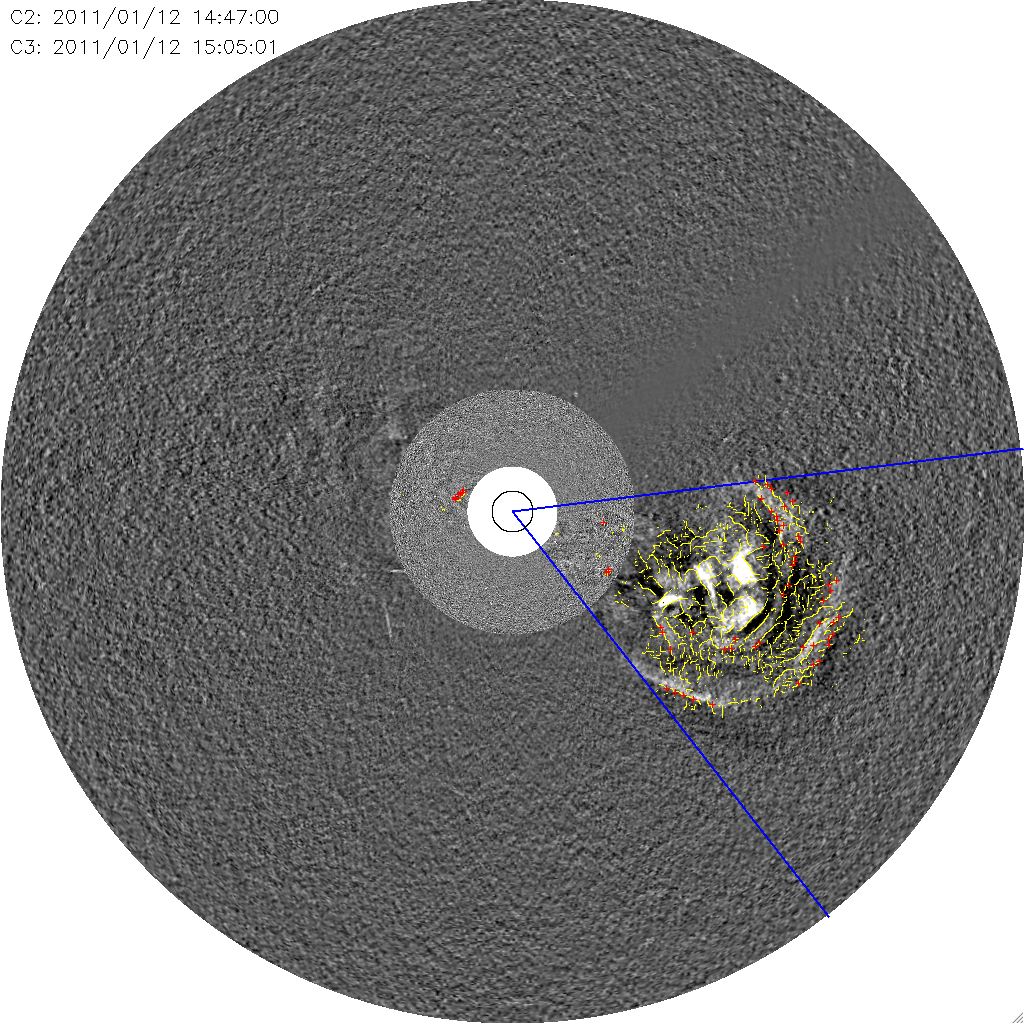
\includegraphics[scale=0.24, trim=0 0 0 0, clip=true]{images/20110112_150501.png}
%\caption{.}
%\label{CMEpng}
%\end{figure}

%\begin{figure}
%\centering
%\includegraphics[scale=0.48, trim=15 0 0 60]{images/plot_kins_quartiles_2011-01-12T11_11_00_sav_gol.eps}
%\caption{The Savitzky-Golay filter applied to the automated CORIMP CME detection and tracking of an event observed on 2011 January 12. The top panel shows the height-time measurements across the angular range of the CME (indicated by the colourbar). The middle and bottom panels show the derived velocity and acceleration profiles, with the median (solid line), interquartile range (inner dashed lines) and upper and lower fences (outer dashed lines) over plotted on the data.}
%\label{fig_savgol_CME_CORIMP}
%\end{figure}

To this end, we shall next investigate a CME that occurred on 2011 January 2, as a case-study from the newly developed CORIMP CME catalogue \citep{2012ApJ...752..144M, 2012ApJ...752..145B}. The height-time points are measured at 1\,degree intervals across the angular span of the event as it moves through the corona in time (see top of Figure~\ref{fig_savgol_CME_CORIMP}). The Savitzky-Golay filer is then applied to each of these angular slices across the CME, and the corresponding first and second order derivatives of the fit are determined. This reveals the spread of velocity and acceleration points as plotted in Figure~\ref{fig_savgol_CME_CORIMP}, with the median, interquartile range, and upper and lower fences over-plotted in order to characterize the significance of the kinematic range. This allows the underlying trend of the data to be inspected, revealing an initial acceleration of approximately $20\,m\,s^{-2}$ up to a constant velocity of approximately $400\,km\,s^{-1}$. Large scatter can inevitably occur at the crossover of the two fields-of-view, and at the outer edge of C3.

Since a spread of measurements across the CME can be determined in these cases, the sample size is therefore larger and the spread is treated as the range of variation in the kinematics without necessarily requiring bootstrap methods to be employed. The implication here is that any variation in CME speeds that may result from the expansion of the ejecta across the plane-of-sky, should provide a distribution of kinematics that is centered on the motion of the bulk of the CME (as opposed to the relatively slower moving flanks of the CME). In essence, this provides a solution space of CME kinematics that is based purely on the distribution of CME height-time measurements. For the automated catalogue, avoiding the need for bootstrapping in this manner also saves on computing time. However, if a user of the catalogue has a specific model that they wish to test against the output, then a bootstrapping procedure and residual analysis would be of use, as demonstrated in Section~\ref{sect:bootstrapping}. Any position angle may be chosen for such analyses, such as the central position angle that may correspond to the maximum speed of the CME. For example, the position angles around $250^{\circ}$ here, indicate speeds up to approximately $500\,km\,s^{-1}$, so for these specific height-time measurements a model may be fit and a bootstrapping technique used to provide a confidence interval for testing the goodness-of-fit. Thus the output produced from this treatment of the kinematics greatly improves the ability to study CME dynamics.

%\begin{table}[ht] 
%\caption{Summary of CME properties as catalogued by the CDAW, CACTus, SEEDS and CORIMP algorithms for comparison.} % title of Table 
%\centering      % used for centering table 
%\begin{tabular}{l c c c c c}
%\hline\hline
%Date & Onset & Pos. & Ang. & Vel. & Accel. \\ % inserts table 
%heading 
%2011-01-02 & time & angle & width & ($km\,s^{-1}$) & ($m\,s^{-2}$) \\ [0.5ex] % inserts table 
%\hline        % inserts single horizontal line 
%CDAW & 15:24 & 268 & 101 & 355 & 21  \\   % inserting body of the table 
%CACTus & 15:48 & 264 & 86 & 264 & 0  \\ 
%SEEDS & 15:36 & 263 & 64 & 244 & 16.6 \\
%CORIMP & 15:55 & 255 & 65 & 167 & 4 \\  [1ex]       % [1ex] adds vertical space 
%\hline     %inserts single line 
%\end{tabular}
%\label{table:catalogues}  % is used to refer this table in the text 
%\end{table}





\subsection{Coronal wave kinematics}
\label{subsect:corpita}

\begin{figure}
\centering
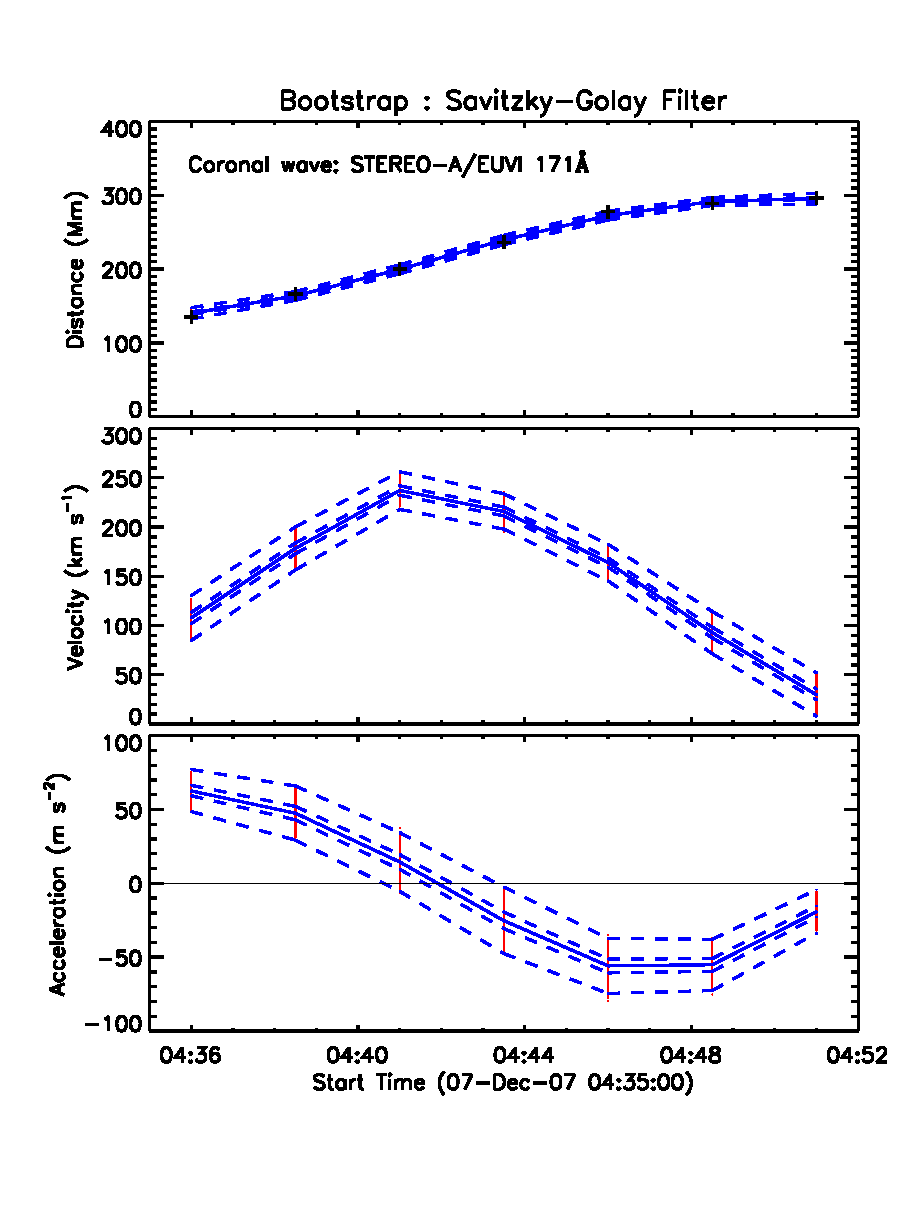
\includegraphics[scale=0.6, trim=0 40 0 30]{images/fit_kinscasestudy_wave20071207.eps}
\caption{The bootstrapped Savitzky-Golay filter method applied to a coronal wave event observed by STEREO-Ahead EUVI-171 on 2007 December 7, revisited from \citet{2011A&A...531A..42L}. The top panel shows the distance-time measurements (\emph{plus symbols}), the resampled residuals (\emph{red points}), and the median (\emph{solid line}), interquartile range (\emph{inner dashed lines}), and upper and lower fences (\emph{outer dashed lines}). The middle and bottom panels show the corresponding velocity and acceleration profiles.}
\label{fig_savgol_wave}
\end{figure}


\begin{figure}[!t]
\centering
\subfigure{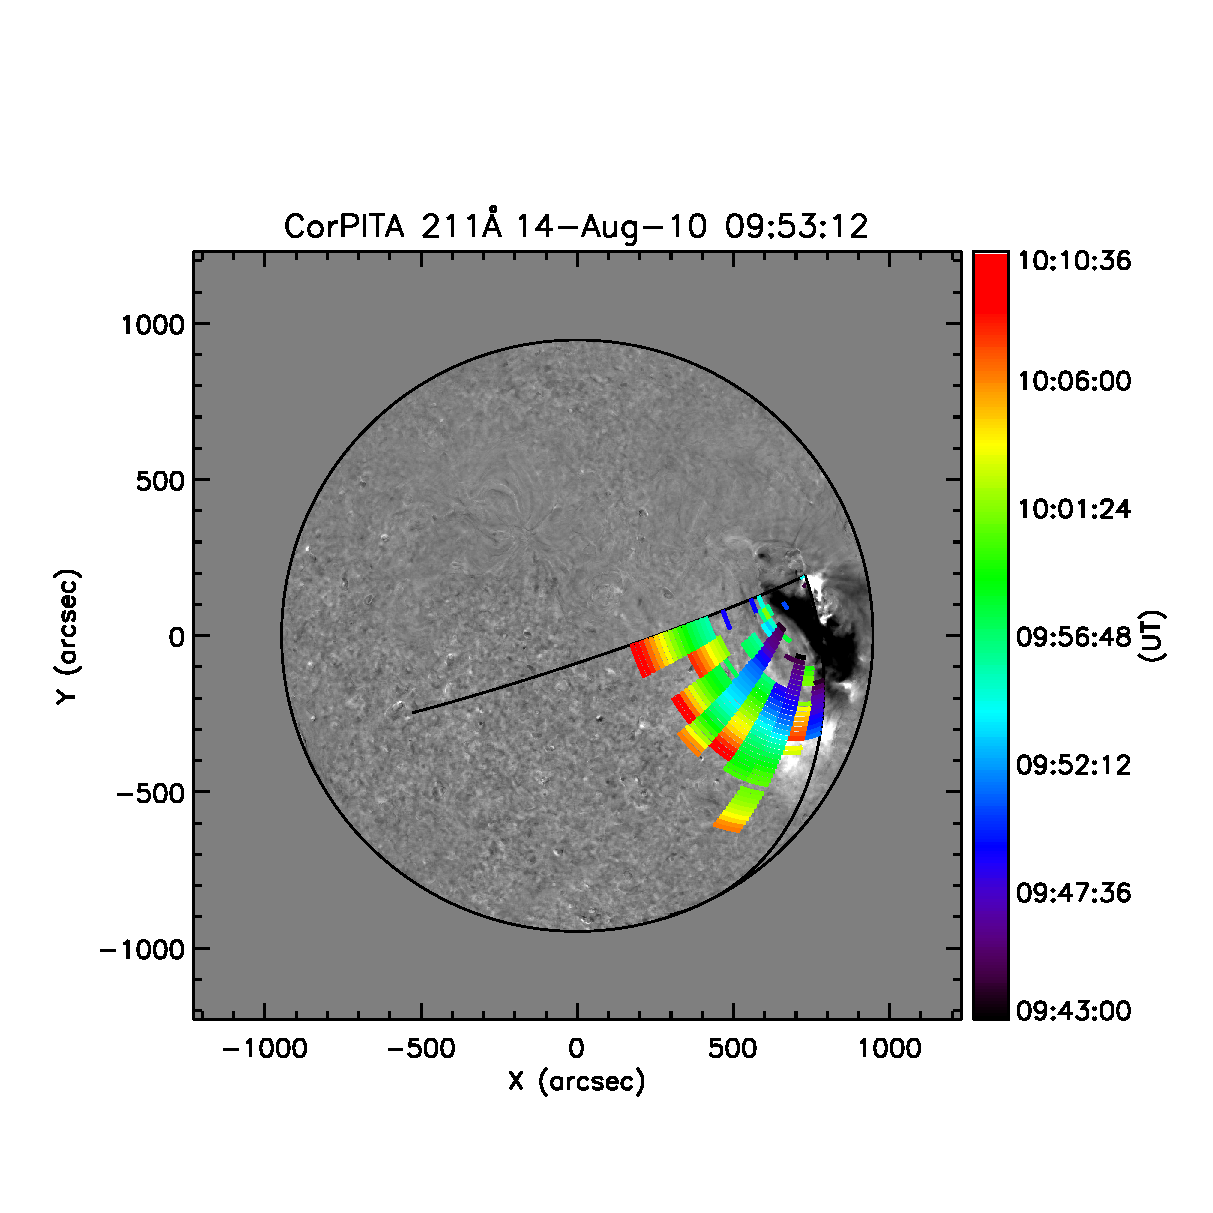
\includegraphics[scale=0.44, trim=10 60 0 70]{images/CorPITA_pulse_20100814_evt.eps}}
\subfigure{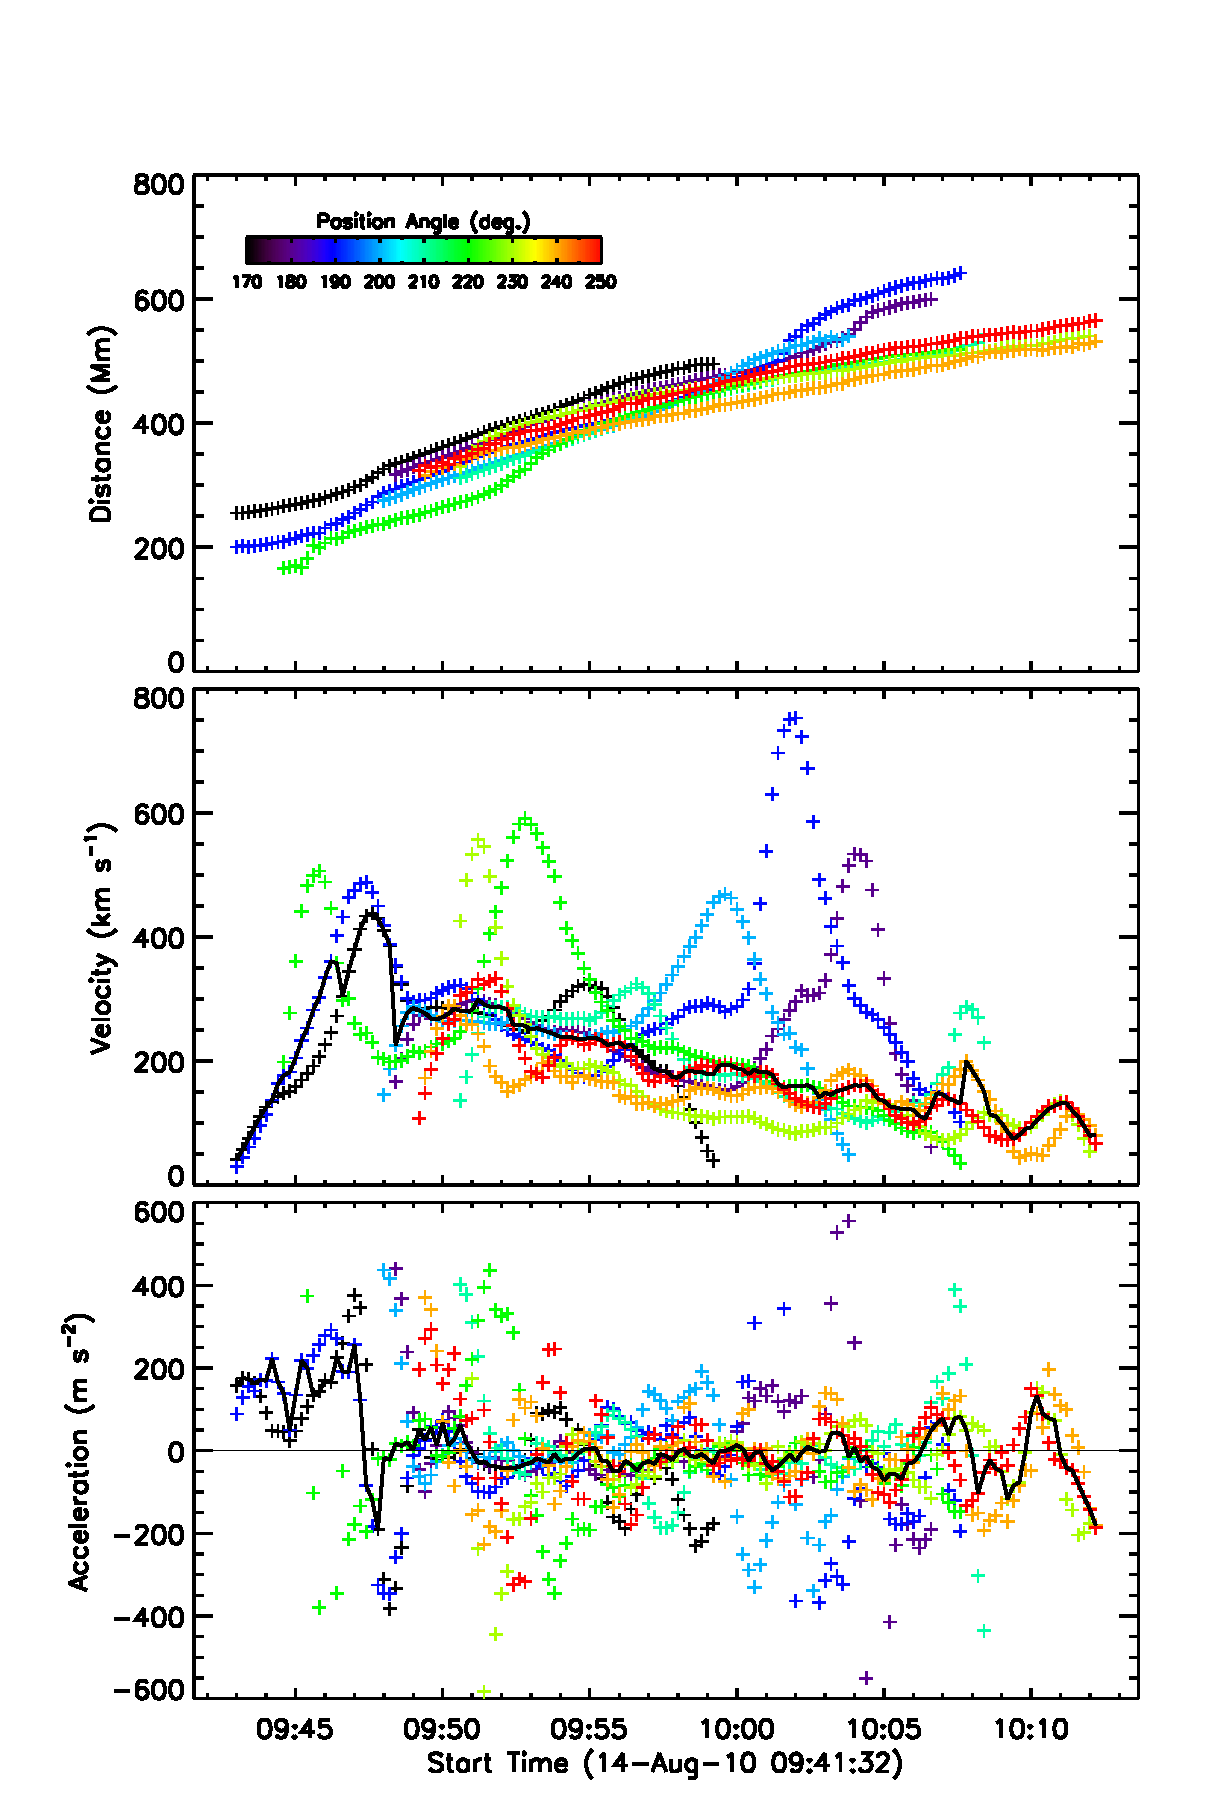
\includegraphics[scale=0.46, trim=10 10 0 70]{images/plot_kins_wave_20100814_savgol.eps}}
\caption{The Savitzky-Golay filter applied to the automated CorPITA detection and tracking of a coronal wave observed by SDO/AIA on 2010 August 14. The top image shows a percentage base differenced frame during the event, with an overlay of the detected wave motion in time. The top panel of the lower plot shows the distance-time measurements across the angular range of the coronal wave. The middle and bottom panels show the derived velocity and acceleration profiles, with the median (\emph{solid line}) over-plotted.}
\label{fig_savgol_wave_CorPITA}
\end{figure}

The treatment of coronal wave kinematics is very similar to that of CMEs, in that a small sample size of distance measurements is obtained, being prone to the effects of scatter from observational and algorithmic biases. We first revisit a coronal wave event studied by \citet{2011A&A...531A..42L}, that was observed by STEREO-A/EUVI-171 on 2007 December 7. In that study, the coronal wave was detected via an intensity thresholding technique on percentage base difference images. Distance-time measurements were produced and studied with a quadratic model of the form of Equation~\ref{eqn:const_a}. Here, we use the Savitzky-Golay filter and bootstrapping technique, as in the CME case study of Figure~\ref{fig_savgol_CME}. The filter width was reduced to operate on 4 neighbouring datapoints (2 either side) since the sample size itself is so small, consisting of only 7 measurements. The top panel of Figure~\ref{fig_savgol_wave} shows the distance-time plot of the coronal wave (the plus symbols), the resampled residuals (in red) after applying the Savitzky-Golay filter, and corresponding median, interquartile range, and upper and lower fences on the bootstrapped data (blue lines). The middle and bottom panels show the derived velocity and acceleration profiles. The kinematic trend strongly implies an initial acceleration of approximately $60\,m\,s^{-2}$, followed by deceleration to $-50\,m\,s^{-2}$, as it then approaches zero velocity. Care must be taken when interpreting this trend from such a small dataset, and such trends would be better justified with increased imager cadences, as is now possible with SDO/AIA for example.

The benefit of a higher cadence was demonstrated in Figure~\ref{cad_hist_weight} for the 12 second cadence of AIA, and since the resolution of the images is also significantly higher than previous missions, the determination of the true kinematics should be greatly improved as a result (c.f. Figure~\ref{noise_test_image}). A coronal wave event observed by AIA, and tracked via the automated CorPITA algorithm, is shown in Figure~\ref{fig_savgol_wave}. The plots show the distance-time measurements (top panels), and derived velocities (middle panels) and accelerations (bottom panels). The Savitzky-Golay filter was again deemed optimal for determining the kinematics of the event, at a filter width of 10 neighbouring datapoints (5 either side). Similar to the previous CME case, this provides a spread of kinematics that is centered on the motion of the bulk of the event, though in this case the measurements were taken at 10 degree intervals, giving a smaller dataset. Therefore, only the median is over-plotted on the velocities and accelerations (without a need for the interquartile ranges or fences). The trend indicates an initial acceleration of approximately $200\,m\,s^{-2}$, attaining speeds of approximately $400\,km\,s^{-1}$ before slowing down. Again, any position angle may be chosen for specific investigation, as described for the previous CME case above. This provides the opportunity to study coronal wave dynamics with improved accuracy and reliability.


\section{Conclusions}
\label{sect:conclusions}

We have demonstrated the unreliability of some common approaches to studying the kinematics of large scale dynamic features in the solar corona, such as CMEs and coronal waves. The dynamics of these phenomena are of great consequence to understanding the physics governing their initiation and propagation, and so the drawbacks of traditional numerical techniques for deriving their velocities and accelerations have been highlighted, and efforts to overcome them discussed. Of particular note on this, is the counter-intuitive behavior of the error propagation in the standard 3-point Lagrangian interpolation, due to its inverse dependence on the observing cadence. It is also shown how strongly affected it can be by noise levels akin to those found in the datasets of these events. Therefore, we outline a somewhat two-fold approach.

Firstly, we suggest the use of bootstrapping techniques when dealing with the small sample sizes of these events, and demonstrate both their ease of implementation, and usefulness in measuring the confidence intervals on fit parameters. It is an effective method for overcoming the limitation of having only a single set of observations of a phenomenon (as is the case for the dynamic events studied here). As a class of resampling methods, bootstrapping allows the construction of a number of resamples of the observed data, from which a distribution of fitting parameters may be generated. Thus the most likely parameter values and associated uncertainties may be determined. Accurate uncertainty intervals are crucial for determining the appropriateness of any chosen theoretical model seeking to characterize the physics of their motion. When used in conjunction with residual analysis, a robust estimate of the goodness-of-fit can be obtained, as demonstrated in Figures~\ref{fig_quadratic} and \ref{fig_savgol}. This is because bootstrapping itself cannot be applied blindly, which leads us to the next point.

Secondly, we suggest that the events may be treated with a priori knowledge, since there is a physical basis for their behavior that can be confidently assumed to a certain extent. For example, the plasma is known to start from rest, and thus undergo an early acceleration to reach its maximum speed. What remains to be tested is exactly the form of that initial acceleration phase, if unexpected trends or changes occur in its motion, and whether additional effects such as from drag and/or interactions with other features of the surrounding environs come in to play. The interpretation of the measurements must also allow for unknown biases that can occur, either due to observational uncertainties (e.g., low intensity profiles embedded in background noise) or algorithmic uncertainties (e.g., erroneous scatter derived at the boundary between instrument fields-of-view). Thus, while the uncertainty of a measurement might be mathematically sound, the measurement itself could be offset in a manner the user must aim to interpret appropriately in the derived kinematics, as demonstrated in Figure~\ref{fig_savgol_CME}.

Many of the issues of traditional numerical differencing techniques and standard error propagation can be overcome by the use of more appropriate methods. Thus we may improve the determination of CME and coronal wave kinematics, and indeed this extends to any similar scenario of a dynamic event. We note that the significance attributed to the kinematic profiles must still be interpreted with care, relying on a priori knowledge so that none of these techniques be blindly applied or interpreted. This is essentially the idea behind Bayesian inference, wherein the probability of a hypothesis is updated as additional evidence is learned. Techniques derived from Bayesian statistics may prove useful for studying the kinematics of solar dynamic phenomena, as observations and catalogues of their properties are built-up over time. For example, \citet{2010SoPh..262..495B} employ a Kalman filter in their development of a dynamic model for three-dimensional tomography of the solar corona. This particular type of algorithm operates recursively over two steps of prediction and update, to build an estimate of the state of a system and associated uncertainties, having prior knowledge of the state of the system. Such approaches may hold promise if they can be adapted for the treatment of solar event kinematics.


\begin{acknowledgements}
This work is supported by SHINE grant 0962716 and NASA grant NNX08AJ07G to the Institute for Astronomy. The SOHO/LASCO data used here are produced by a consortium of the Naval Research Laboratory (USA), Max-Planck-Institut fuer Aeronomie (Germany), Laboratoire d'Astronomie (France), and the University of Birmingham (UK). SOHO is a project of international cooperation between ESA and NASA. SDO data supplied courtesy of the NASA/SDO consortia. The STEREO/SECCHI project is an international consortium of the Naval Research Laboratory (USA), Lockheed Martin Solar and Astrophysics Lab (USA), NASA Goddard Space Flight Center (USA), Rutherford Appleton Laboratory (UK), University of Birmingham (UK), Max-Planck-Institut f\"{u}r Sonnen-systemforschung (Germany), Centre Spatial de Liege (Belgium), Institut d'Optique Th\'{e}orique et Appliqu\'{e}e (France), and Institut d'Astrophysique Spatiale (France). The authors would like to acknowledge the help and guidance from the SDO Feature Finding Team. DL would like to thank the Institute for Astronomy at the University of Hawaii for their generous hospitality. 
\end{acknowledgements}



\bibliographystyle{apj.bst}
\bibliography{references.bib}  



\end{document}